\newcommand{\triangOK}{\textcolor[rgb]{00,0.45,0.10}{$\blacktriangle$}}
\newcommand{\triangBAD}{\textcolor[rgb]{0.7,00,00}{$\blacktriangledown$}}
\newcommand{\ball}{\textcolor[rgb]{0.7,0.70,0.0}{$\bullet$}}

\definecolor{Gray}{gray}{0.9}
\definecolor{LightCyan}{rgb}{0.90,0.9,1}

%\begin{table}
%\centering
%\caption{}
%\label{tab::}
%\begin{footnotesize}
%\toprule
%Tabela
%\midrule
%\bottomrule
%\end{footnotesize}
%\end{table}

\chapter{Experimentos}
\label{cap::experimentos}

Nesse capítulo relatamos os diversos experimentos efetuados para testar a eficácia dos métodos para estimar a credibilidade de exemplos. % e seus resultados.
Decidimos por realizar a divisão desse capítulo em seis partes.
Na primeira, a Seção~\ref{subsec::base}, mostramos as várias bases de dados que usamos em nossos experimentos.
Depois, mostramos na Seção~\ref{subsec::gpparam} os diversos parâmetros utilizados pelo \textsc{PG}, incluindo sua função de \textit{fitness}.
Já a Seção~\ref{subsubsec::cv} aborda a metodologia usada para realização dos testes.
%Por fim, nas três últimas seções exibimos os resultados dos três tipos de base usadas, documentos (Seção~\ref{sec::documentos}), categorias (Seção~\ref{sec::categorias}) e bioinformática (Seção~\ref{sec::bioinfo}).
%
%abordamos alguns pontos em comum de todos os experimentos, como a metodologia da Validação Cruzada, os parâmetros do \textsc{PG} e a função de \textit{fitness} empregada, além de.
Nas Seções~\ref{sec::documentos} e \ref{sec::categorias}, abordamos a classificação com a utilização de funções credibilidade em atributos textuais e categóricos, respectivamente.
Os atributos textuais provêm de bases de documentos muito utilizadas na literatura, em especial a base da \textsc{ACM-DL}, que contém também informações usadas para credibilidade de relacionamentos.
Por sua vez, os atributos categóricos vêm de bases do \textsc{UCI}.
Finalmente, na Seção~\ref{sec::bioinfo}, apresentamos os resultados provenientes de utilizar a classificação de atributos numéricos e as funções de credibilidade de relacionamentos em uma base de assinaturas estruturais proteicas.

%%%%%%%%%%%%%%%%%%%%%%%%%%%%%%---------------------------------------------------%%%%%%%%%%%%%%%%%%%%%%%%%%%%%%
%%%%%%%%%%%%%%%%%%%%%%%%%%%%%%%---------------------------------------------------%%%%%%%%%%%%%%%%%%%%%%%%%%%%%%
%%%%%%%%%%%%%%%%%%%%%%%%%%%%%%%--------------        5.1          ----------------%%%%%%%%%%%%%%%%%%%%%%%%%%%%%%
%%%%%%%%%%%%%%%%%%%%%%%%%%%%%%%---------------------------------------------------%%%%%%%%%%%%%%%%%%%%%%%%%%%%%%
%%%%%%%%%%%%%%%%%%%%%%%%%%%%%%%---------------------------------------------------%%%%%%%%%%%%%%%%%%%%%%%%%%%%%%


\section{Bases de Dados}
\label{subsec::base}

Nosso trabalho se divide em três tipos de bases de dados: as bases de documentos, as bases do \textsc{UCI} (\cite{UCI98}) e uma base de bioinformática.

Iniciamos descrevendo as quatro bases de documentos: \textsc{ACM-DL}, \textit{Reuters}, \textit{Ohsumed} e \textit{20-newsgroup}.
%mostrar a Figura \ref{fig::basesdoc}, contendo as distribuições dos exemplos das quatro bases de documentos que estamos usando.
 Todas elas foram pré-processadas, com remoção de \textit{stop words} e \textit{steming}, assim como foi atribuída somente uma única classe para todos os documentos que originalmente poderiam pertencer a mais de uma.

A base de documentos digitais da \textsc{ACM}, chamada \textsc{ACM-DL} (\textit{Association for Computing Machinery Digital Library}), é um rico acervo de artigos acadêmicos da área da Ciência da Computação. Utilizamos somente um subconjunto da base, formado por 56.450 termos encontrados em 24.897 artigos divididos em 11 classes.
A base da \textsc{ACM} é a única que apresenta informações sobre os autores e citações contidas nos seus documentos.
Podemos criar dois grafos de relacionamentos com essas informações: um para os autores e outro para as citações.
Ao todo o grafo de autoria tem 16.005 vértices (documentos) e 72.645 arestas, sendo que cada aresta representa o número de autores em comum dois documentos possuem.
Já o grafo de citações tem 31.482 vértices e 95.812 arestas, onde os vértices são documentos e as arestas são direcionadas e significam que um documento cita o outro.
Observe que o número de documentos no grafo de citações é maior que o número de artigos existentes no subconjunto da \textsc{ACM-DL}. Isso acontece porque estamos usando um subconjunto dos documentos da \textsc{ACM-DL} e ele contém informações sobre artigos que estão fora desse subconjunto. Para ser mais exato, apenas 5.305 artigos do grafo de citação estão presentes na base que usamos, enquanto os outros 26.176 não estão.

A base \textit{Reuters}, por sua vez, contém 8.184 documentos divididos em 8 classes, e 24.986 termos distintos. Os documentos são provenientes da agência de notícias com o mesmo nome da base.
Já a base \textit{Ohsumed} apresenta 18.302 documentos médicos divididos em 23 classes e 45.991 termos.
Finalmente, a base 20-\textit{newgroup} (\textit{20ng}) contém 18.827 mensagens de texto com 110.502 termos únicos, enviadas para grupos de notícia de diversos assuntos como ciência, religião, entre outros, totalizando 20 classes.

A Figura~\ref{fig::basesdoc} mostra a distribuição exemplos/classe das bases citadas acima.
Todos os pontos mostrados na Figura \ref{fig::basesdoc} são referentes à quantidade de exemplos de cada classe, ordenados de maneira crescente, da classe de menor popularidade para a de maior. Verificamos que a base \textit{20-newsgroup} é a que apresenta a distribuição mais equilibrada de exemplos por classe, enquanto a \textit{Ohsumed} apresenta a pior, com 17 das 23 classes contendo menos que 1.000 exemplos por classe e com duas classes contendo mais de 2.500.

\begin{figure}[!h]
  \centering
  \subfloat[][ACM-DL]{\label{fig::acm}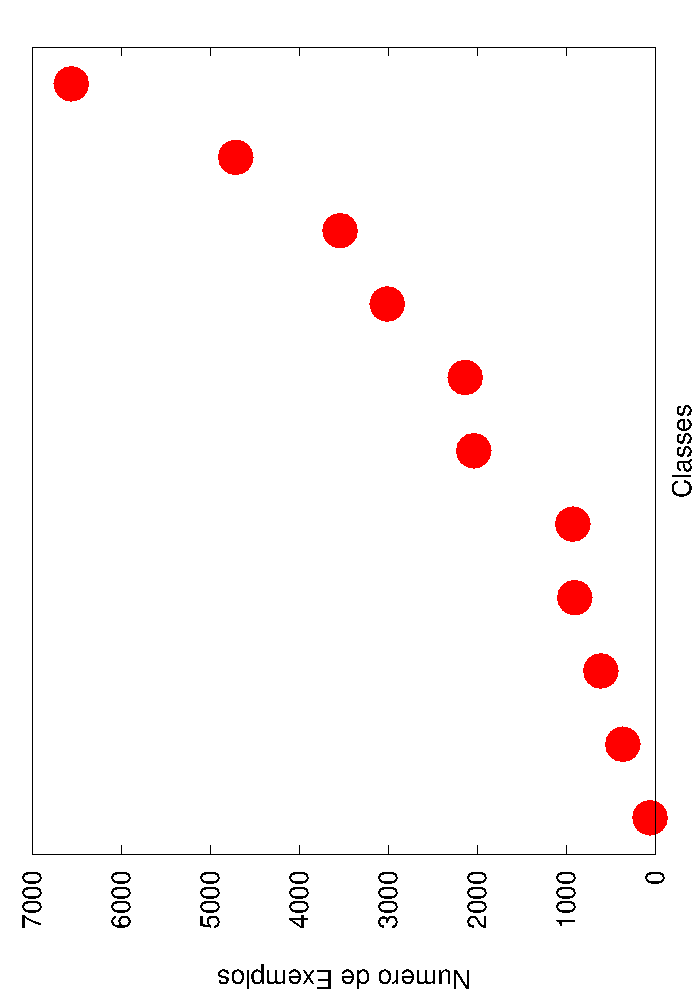
\includegraphics[angle=270, width=0.40\textwidth]{figures/perfil/acm.png}}
  \subfloat[][Reuters]{\label{fig::reuters}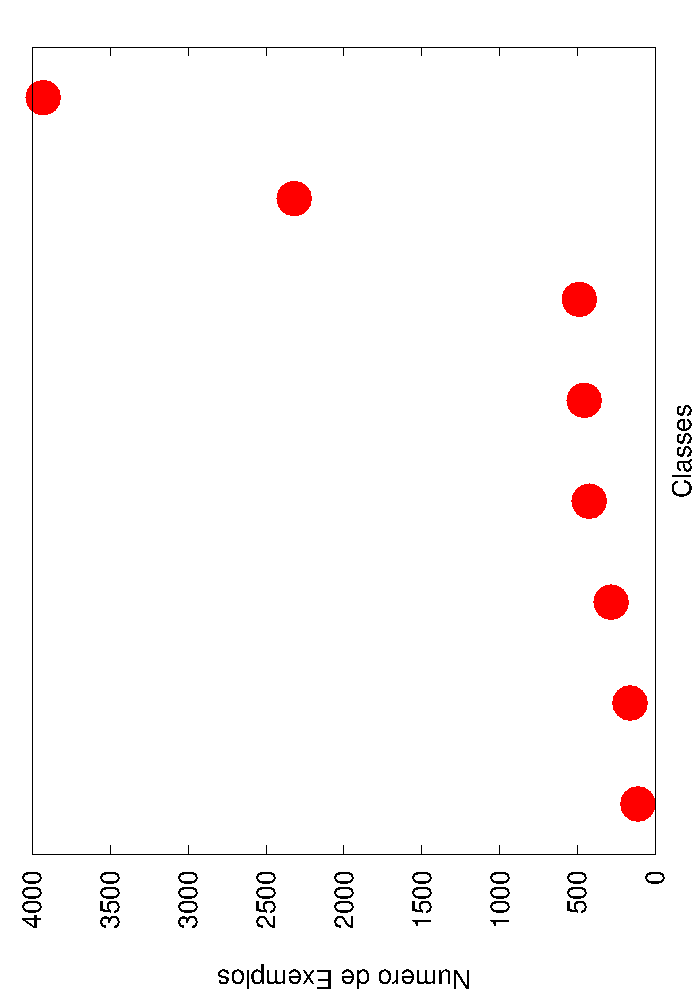
\includegraphics[angle=270, width=0.40\textwidth]{figures/perfil/reuters.png}}
    \\
  \subfloat[][Ohsumed]{\label{fig::ohsumed}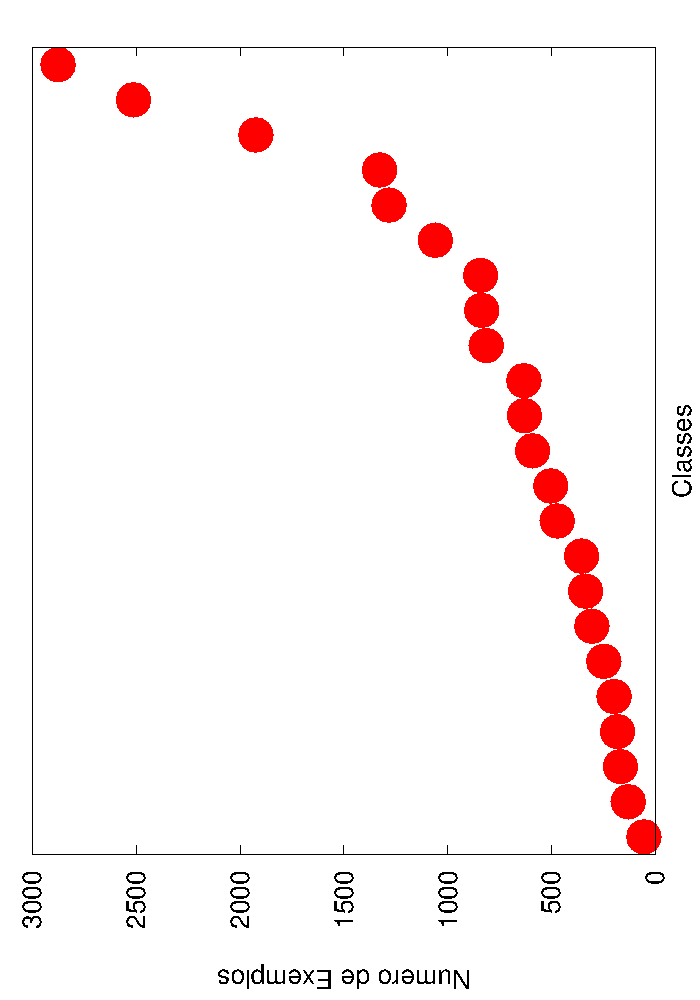
\includegraphics[angle=270, width=0.40\textwidth]{figures/perfil/ohsumed.png}}
  \subfloat[][20-NewsGroup]{\label{fig::20ng}\includegraphics[angle=270, width=0.40\textwidth]{figures/perfil/20ng.png}}

\caption{Distribuição dos exemplos nas classes das bases de documentos.}
\label{fig::basesdoc}
\end{figure}

Já a Figura \ref{fig::basescategorias}, mostra o perfil de quatro bases do repositório de bases para aprendizado de máquina da Universidade da Califórnia em Irvine (\textsc{UCI}). Todas as bases são compostas por poucos atributos, todos categóricos, e poucas classes.
A base \textit{Cars} contém 1.728 exemplos com 6 atributos cada, apresentando características importantes para decidir a condição de um carro usado entre não aceitável, aceitável, bom e muito bom. A base \textit{chess} utiliza 36 atributos e 3.196 instâncias para decidir se a partir de alguns movimentos finais do jogo de xadrez, o jogador que joga com as peças brancas pode ganhar ou não. \textit{Nursery} é uma base formada por candidaturas para as escolas de enfermaria de Liubliana, Eslovênia. Ela é composta de 12.960 exemplos com 8 atributos que descrevem aspectos de um(a) candidato(a) para a escola de enfermaria. Cada exemplo pode ser classificado em cinco classes que vão desde não recomendado até fortemente recomendado, com a classe recomendado apresentando apenas dois exemplos.
Por último, a base \textit{tictactoe} mostra as 958 combinações possíveis das 9 casas do jogo da velha, sendo as classes possíveis a vitória do jogador \textsc{x} ou não.

\begin{figure}[h]
  \centering
  \subfloat[][cars]{\label{fig::cars}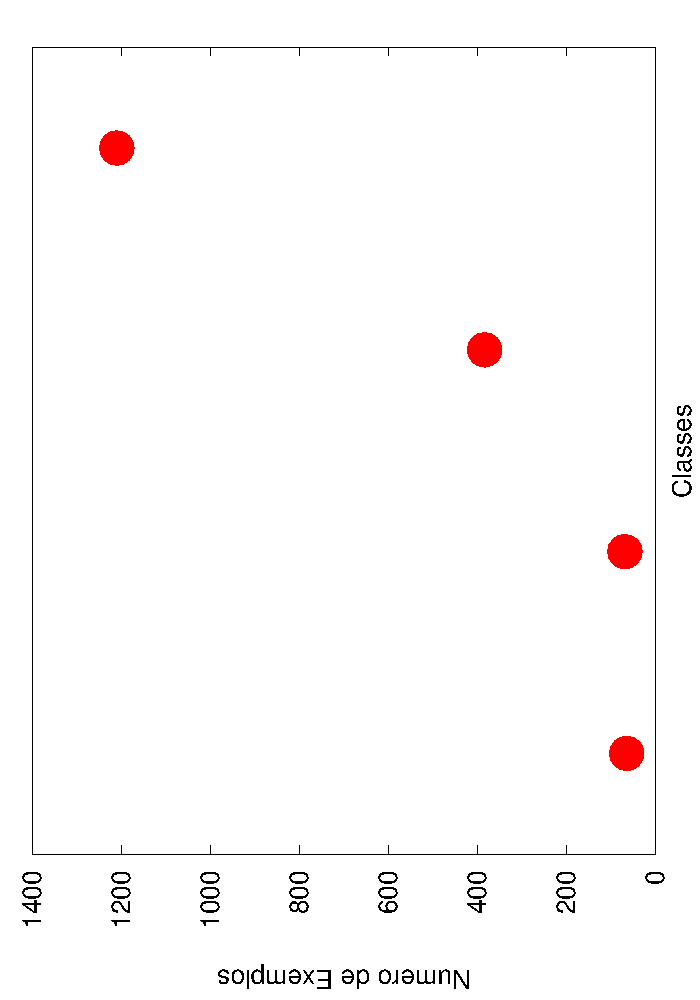
\includegraphics[angle=270, width=0.40\textwidth]{figures/perfil/cars.png}}
  \subfloat[][chess]{\label{fig::chess}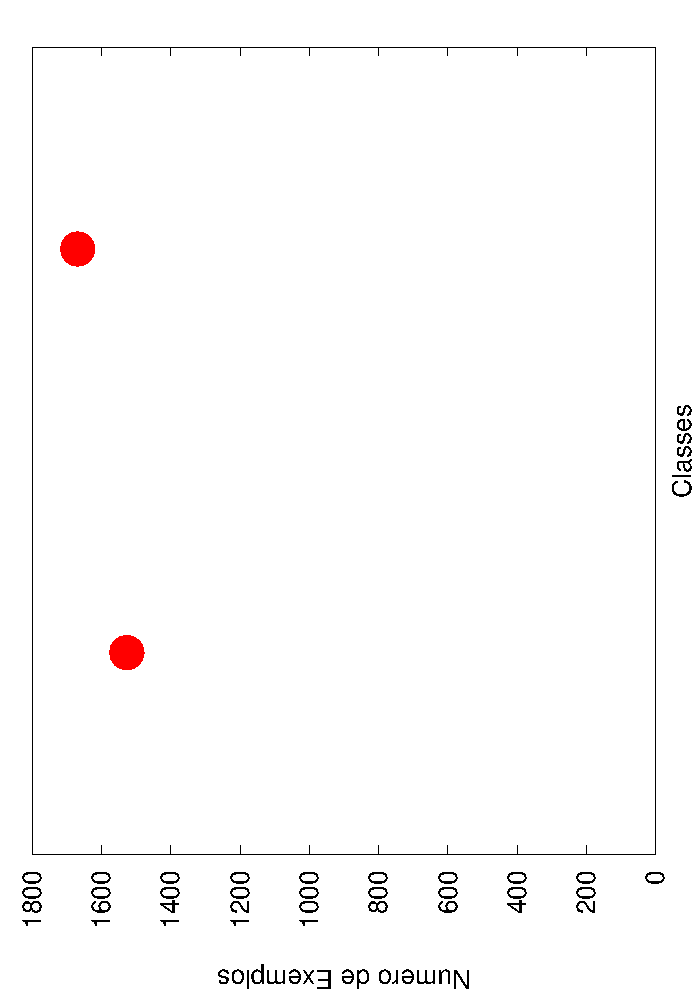
\includegraphics[angle=270, width=0.40\textwidth]{figures/perfil/chess.png}}
    \\
  \subfloat[][nursery]{\label{fig::nursery}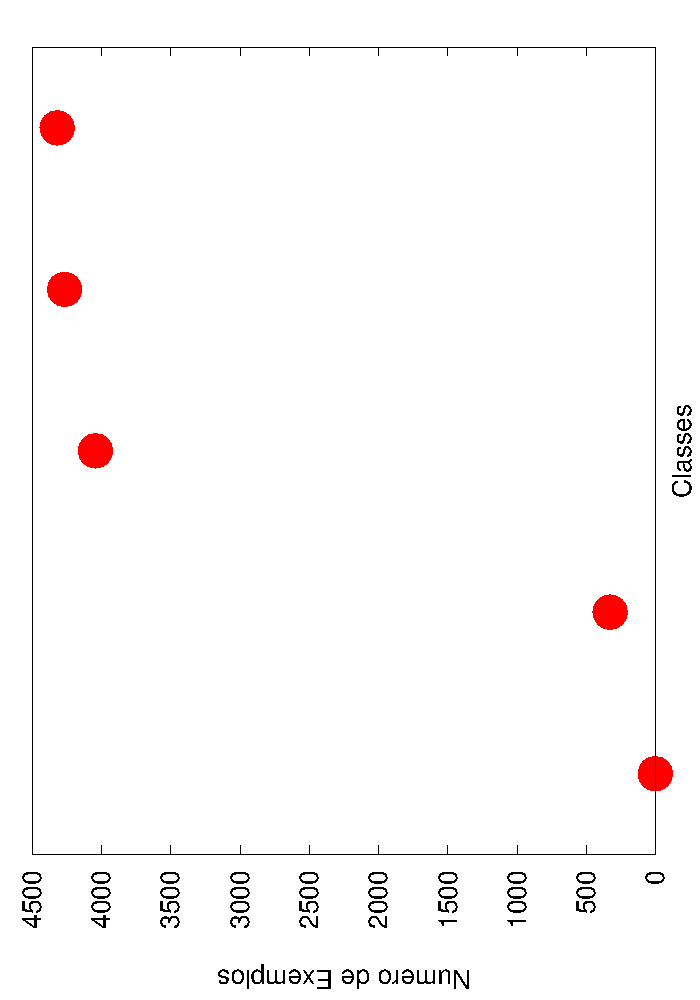
\includegraphics[angle=270, width=0.40\textwidth]{figures/perfil/nursery.png}}
  \subfloat[][tictactoe]{\label{fig::tictactoe}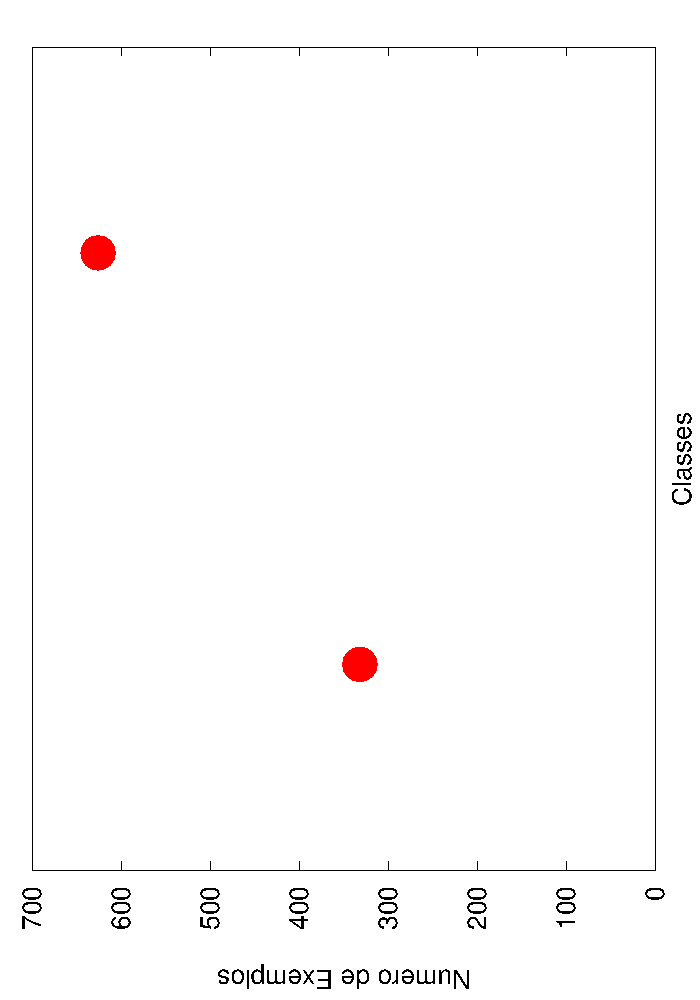
\includegraphics[angle=270, width=0.40\textwidth]{figures/perfil/tictactoe.png}}

\caption{Distribuição dos exemplos nas classes das bases de atributos categóricos.}
\label{fig::basescategorias}
\end{figure}

Finalmente, utilizamos uma base de assinaturas estruturais proteicas, geradas pelo método \textsc{CSM} (\cite{dpires_bmc_2011}) a partir do repositório de domínios proteicos ASTRAL (\cite{Brenner00}).
Ela é utilizada para a tarefa de classificação estrutural de proteínas e usa o nível de família da classificação \textsc{SCOP} (\cite{SCOP95}), que classifica proteínas nos níveis hierárquicos de classe, enovelamento, super família e família, sendo família o nível mais específico e muitas vezes o mais difícil de classificar. Assim como feito em \cite{dpires_bmc_2011}, foi utilizado o método de decomposição por valor singular (\textsc{SVD}) (\cite{SVD}) para reduzir a dimensionalidade e ruídos da base para apenas 15 atributos, tornando a execução dos algoritmos de classificação mais rápida sem grande degradação dos resultados.
Na Figura~\ref{fig::basesbio} vemos como as 110.799 proteínas são distribuídas nas 4.193 classes existentes, sendo que todas as classes têm ao menos dez exemplos.
Nesse domínio exploramos a credibilidade de relacionamentos, onde o relacionamento corresponde a similaridade entre duas sequências proteicas. Essa similaridade é gerada utilizando o método \textsc{BLAST} (\cite{altschul90}). Dessa forma, definimos uma relação entre todos os pares de estruturas presentes na base. Com o intuito de utilizar somente as informações mais relevantes e diminuir o tamanho do grafo gerado, estipulamos um limite inferior de corte de 40\% de similaridade. Ainda assim restaram 11.461.022 ligações entre os exemplos da base.

%Assinaturas estruturais proteicas derivadas (geradas) pelo método CSM

%Base:
%tarefa de classificacao estrutural
%classifiquei no familia SCOP nivel familia.
%SCOP 1.75 da proteinas e assinaturas sao geradas....pelo CSM...

%Grafo:
%para gerar o grafo foi feito um alinhamento par a par das sequencias utilizando o metodo BLAST  , gerando um score de similaridades nas comparacoes entre todos os pares de sequencias proteicas.(ver corte...)

\begin{figure}[!h]
  \centering
%  \subfloat[][Astral]{\label{fig:astral}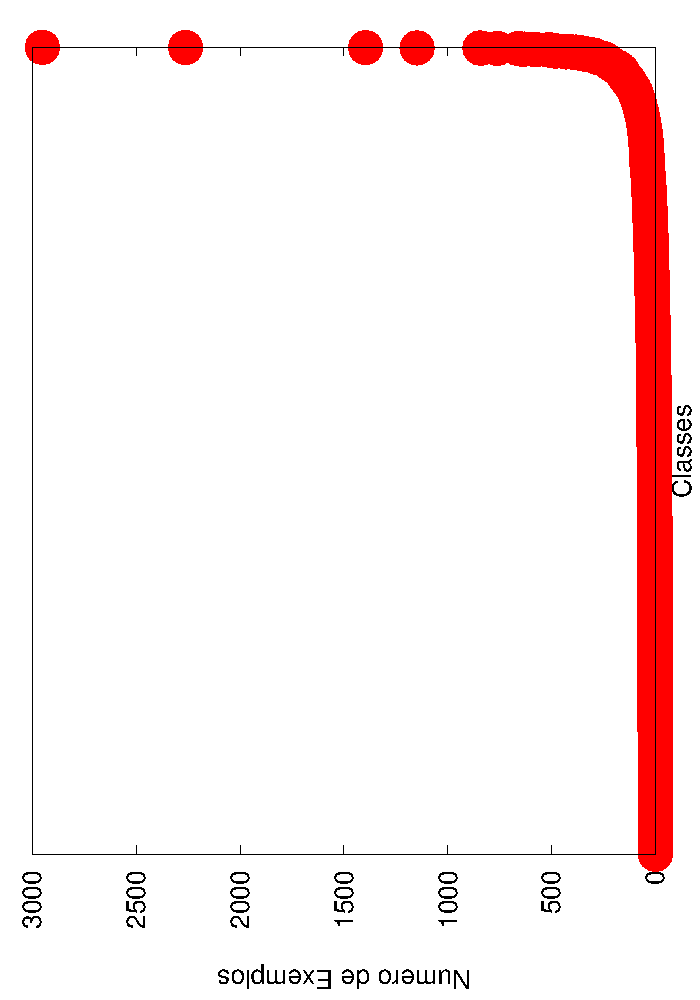
\includegraphics[angle=270, width=0.40\textwidth]{figures/perfil/astral.png}}
%  \subfloat[][Douglas]{\label{fig:douglas}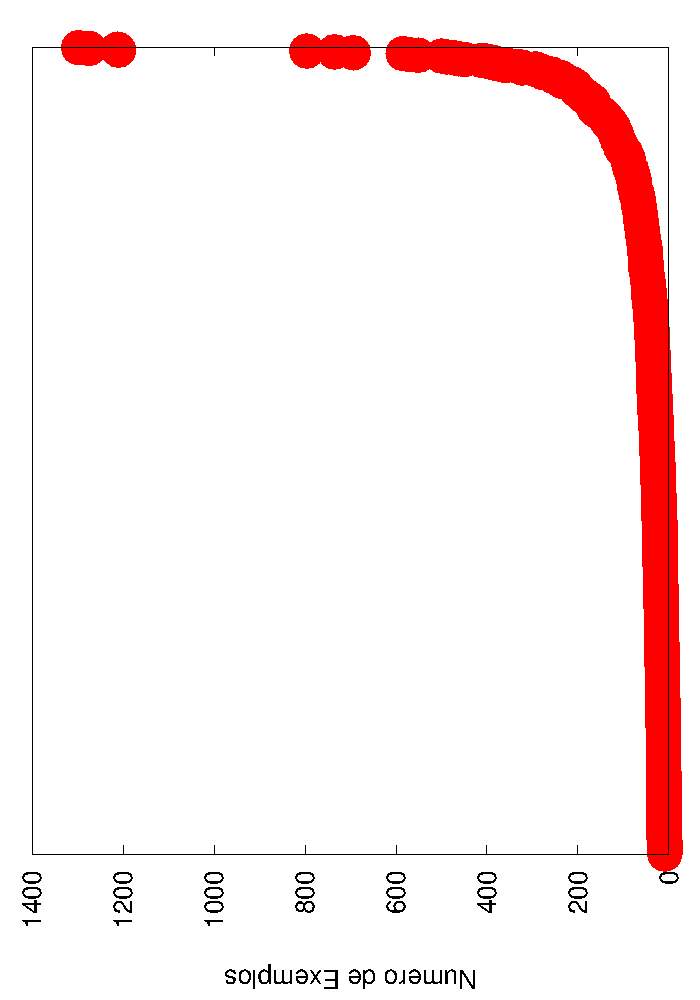
\includegraphics[angle=270, width=0.40\textwidth]{figures/perfil/douglas.png}}
  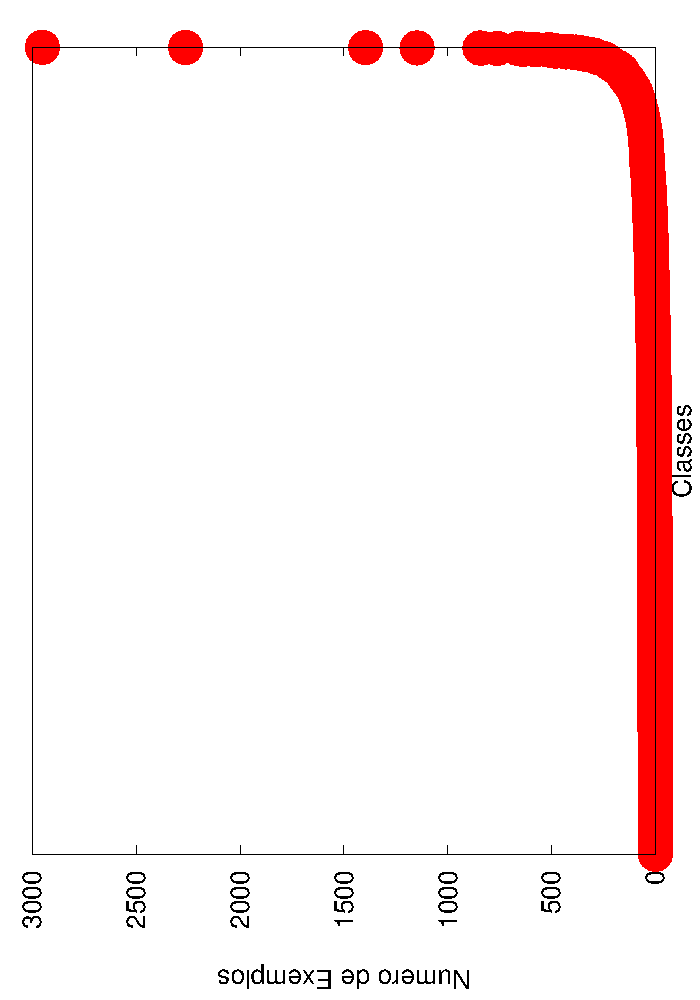
\includegraphics[angle=270, width=0.40\textwidth]{figures/perfil/astral.png}
 \caption{Distribuição dos exemplos nas classes na base de assinaturas estruturais proteicas.}
\label{fig::basesbio}
\end{figure}

%%%%%%%%%%%%%%%%%%%%%%%%%%%%%%%---------------------------------------------------%%%%%%%%%%%%%%%%%%%%%%%%%%%%%%
%%%%%%%%%%%%%%%%%%%%%%%%%%%%%%%---------------------------------------------------%%%%%%%%%%%%%%%%%%%%%%%%%%%%%%
%%%%%%%%%%%%%%%%%%%%%%%%%%%%%%%--------------        5.2          ----------------%%%%%%%%%%%%%%%%%%%%%%%%%%%%%%
%%%%%%%%%%%%%%%%%%%%%%%%%%%%%%%---------------------------------------------------%%%%%%%%%%%%%%%%%%%%%%%%%%%%%%
%%%%%%%%%%%%%%%%%%%%%%%%%%%%%%%---------------------------------------------------%%%%%%%%%%%%%%%%%%%%%%%%%%%%%%


\section{Configuração de Parâmetros}
\label{subsec::gpparam}

A configuração de parâmetros em um algoritmo de Programação Genética é um dos muitos desafios encontrados nesse trabalho. Procuramos utilizar uma combinação que seja boa o suficiente para todos os testes aqui exibidos. Isso quer dizer que poderíamos obter resultados ainda melhores se ajustássemos os parâmetros focando em cada teste, porém iríamos ter dezenas de tabelas de configurações, o que definitivamente não é desejado. Portanto, efetuamos vários testes prévios em todas as bases estudadas para, finalmente, chegarmos aos parâmetros mostrados na Tabela~\ref{tab::parametros}.
Destacamos o uso do programa de visualização chamado Galapagos (\cite{galapagos}), que nesse ano ganhou o prêmio de melhor ferramenta para visualização de algoritmos evolucionários da conferência ACM-Gecco 2011 (\textit{Genetics and Evolutionary Computation Conference}).

\begin{table}[!h]
\centering
\caption{Principais parâmetros utilizados no \textsc{PG}.}
\label{tab::parametros}
\begin{tabular}{|c||c|}
\toprule
\textbf{Parâmetro} & \textbf{Valor}\tabularnewline
\midrule
\hline
Tamanho da População & 100\tabularnewline
\hline
Número de Gerações & 100\tabularnewline
\hline
Tipo de Seleção & Torneio\tabularnewline
\hline
Tamanho do Torneio & 2\tabularnewline
\hline
Probabilidade de Reprodução & 10\%\tabularnewline
\hline
Probabilidade de Cruzamento & 90\%\tabularnewline
\hline
Probabilidade de Mutação & 10\%\tabularnewline
\hline
Tamanho Máximo da Árvore & 6\tabularnewline
%nao sao parametros, sao componentes do metodo
%\hline
%Elitismo & Sim\tabularnewline
%\hline
%Método de Inicialização & \textit{Ramped-Half-and-half}\tabularnewline
\hline
Tamanho Inicial Máximo & 4 \tabularnewline
\bottomrule
\end{tabular}
\end{table}

%[0]  GPVariable Variable growth. During creation, the children of a function node are chosen from either the function set or the terminal set with a certain probability (in this case always 50%).
%[1] GPGrow All branches have a maximum depth.
%[2] GPRampedHalf Koza uses this creation method. It is half and half of GPRampedVariable and GPRampedGrow.
%[3] GPRampedVariable Ramped means that during creation, the allowable tree depth is increased up to the maximum specified by the user. The behaviour is the same as GPVariable otherwise.
%[4] GPRampedGrow Same as GPGrow except for the maximum allowable tree depth which changes according to a ramp during creation.
%[5] GPUserDefinedCreation This is not implemented, but the user can do this in one of his inherited classes.

Como mostrado no Capítulo~\ref{cap::programacao_genetica}, o parâmetro ``tamanho da população'' controla quantos indivíduos teremos em cada uma das gerações e o ``número de gerações'' define até quando o \textsc{PG} evoluirá. Como já falamos também, utilizamos a seleção por torneios formados por apenas dois indivíduos, evitando assim a convergência prematura do algoritmo.
Mostramos também os diversos valores de probabilidade para a criação da população da próxima geração. 

Além disso, três importantes configurações aparecem nas últimas linhas da tabela. Na antepenúltima linha, exibimos que estamos usando a técnica chamada elitismo, na qual o melhor indivíduo de cada geração é automaticamente reproduzido na próxima geração. Finalmente, na última linha, temos o parâmetro utilizado pelo método de inicialização do \textsc{PG}. Ele força que metade da população tenha um tamanho inicial \textbf{igual} ao tamanho inicial máximo, ou seja, quatro, e que a outra metade tenha um tamanho inicial de \textbf{no máximo} o tamanho inicial máximo.


Além dos parâmetros convencionais apresentamos também resultados de experimentos preliminares que determinam a \textit{fitness} do algoritmo.
Como apontado na Seção~\ref{subsec::fitness}, a \textit{fitness} desempenha importante papel em um algoritmo de Programação Genética, pois define quem são os melhores indivíduos, sendo um importante meio para compará-los.
Usualmente, os trabalhos de classificação presentes na literatura reportam a Micro e Macro-$F_1$, pelo papel que apresentam em tentar balancear a taxa de acerto com uma boa cobertura, medindo a capacidade do classificador prever corretamente indivíduos em todas as classes.

Em nossos trabalhos passados (\cite{Palotti10,Palotti11})
e nos experimentos aqui presentes, utilizamos a Micro-$F_1$ como função de \textit{fitness}, pois é mais comum encontrar trabalhos na literatura reportando a Micro-$F_1$ do que a Macro-$F_1$. Entretanto, é interessante investigar quais são os resultados obtidos por alterar a função de \textit{fitness}, substituindo a Micro-$F_1$ pela (i) Macro-$F_1$ e (ii) pela soma das duas.

Nas Tabelas~\ref{tab::fitness-micro} e \ref{tab::fitness-macro}, mostramos os resultados da Micro$F_1$ e Macro$F_1$, respectivamente, ao aplicar as três funções de \textit{fitness} propostas.
A utilização da \textit{fitness} = Micro$F_1$ serve como linha de base e informarmos os ganhos nas duas últimas colunas relativos a ela.
Assim como em várias da tabelas presentes nesse capítulo, usamos 3 símbolos: \triangOK, \triangBAD, \ball, para dizer, respectivamente, que temos uma comparação significativamente melhor, pior ou impossível de se afirmar de acordo com um teste de hipóteses (\textit{test-t}) com nível de confiança de 99\%.


\begin{table}[h]
\centering
\caption{Experimentos mostrando a micro$F_1$ ao variar a função de \textit{fitness}.}
\label{tab::fitness-micro}
\begin{footnotesize}
\begin{tabular}{|c||c|c|c|}
\toprule
\multirow{2}{*}{\textbf{Bases}} & \multicolumn{3}{c|}{\textbf{Função de Fitness}}\tabularnewline
\cline{2-4} 
 & \textbf{Micro$F_1$} & \textbf{Macro$F_1$} & \textbf{Micro$F_1$ + Macro$F_1$}\tabularnewline
\midrule
\hline
ACM & 74.33 \textpm{} 0.72 & 72.96 \textpm{} 0.98 (-1.84 \triangBAD) & 73.99 \textpm{} 0.80 (-0.45 \ball)\tabularnewline
\hline 
20ng & 89.06 \textpm{} 0.15 & 87.92 \textpm{} 1.59 (-0.01 \ball) & 87.65 \textpm{} 2.12 (-0.32 \ball)\tabularnewline
\hline 
Ohsumed & 69.34 \textpm{} 0.55 & 68.83 \textpm{} 1.47 (-0.73 \ball) & 69.76 \textpm{} 1.19 (0.60 \ball)\tabularnewline
\hline 
Reuters & 94.60 \textpm{} 0.44 & 93.96 \textpm{} 0.75 (-0.67 \ball) & 94.59 \textpm{} 0.50 (-0.01 \ball)\tabularnewline
\bottomrule
\end{tabular}
\end{footnotesize}
\end{table}


\begin{table}[h]
\centering
\caption{Experimentos mostrando a macro$F_1$ ao variar a função de \textit{fitness}.}
\label{tab::fitness-macro}
\begin{footnotesize}
\begin{tabular}{|c||c|c|c|}
\toprule
\multirow{2}{*}{\textbf{Bases}} & \multicolumn{3}{c|}{\textbf{Função de Fitness}}\tabularnewline
\cline{2-4} 
 & \textbf{Micro$F_1$} & \textbf{Macro$F_1$} & \textbf{Micro$F_1$ + Macro$F_1$}\tabularnewline
\midrule
\hline
ACM & 59.72 \textpm{} 1.26 & 60.03 \textpm{} 1.45 (0.52 \ball) & 60.20 \textpm{} 1.54 (0.81 \ball)\tabularnewline
\hline 
20ng & 88.69 \textpm{} 0.22 & 86.46 \textpm{} 3.80 (-1.06 \ball) & 87.11 \textpm{} 2.47 (-0.32 \ball)\tabularnewline
\hline 
Ohsumed & 63.56 \textpm{} 0.89 & 63.62 \textpm{} 1.88 (0.10 \ball) & 64.38 \textpm{} 1.91 (1.30 \ball)\tabularnewline
\hline 
Reuters & 89.33 \textpm{} 0.90 & 88.04 \textpm{} 0.73 (-1.44 \triangBAD) & 89.08 \textpm{} 0.83 (-0.28 \ball)\tabularnewline
\bottomrule
\end{tabular}
\end{footnotesize}
\end{table}

%\begin{table}[h]
%\centering
%\caption{Experimentos mostrando a micro$F_1$ variando a função de \textit{fitness}.}
%\label{tab::fitness-micro}
%\begin{footnotesize}
%\begin{tabular}{|c|c|c|c|c|}
%\toprule
%\multirow{2}{*}{\textbf{Bases}} & \multirow{2}{*}{\textbf{Linha de Base}} & \multicolumn{3}{c|}{\textbf{Funcão de Fitness}}\tabularnewline
%\cline{3-5} 
% &  & \textbf{Micro$F_1$} & \textbf{Macro$F_1$} & \textbf{Macro$F_1$ + Micro$F_1$}\tabularnewline
%\midrule
%ACM & 73.63 \textpm{} 0.91 & 74.33 \textpm{} 0.72 (0.95 \ball) & 72.96 \textpm{} 0.98 (-0.91 \ball) & 73.99 \textpm{} 0.80 (0.49 \ball)\tabularnewline
%\hline 
%20NG & 84.94 \textpm{} 0.58 & 89.06 \textpm{} 0.15 (4.85 \triangOK) & 87.92 \textpm{} 1.59 (3.61 \triangOK) & 88.71 \textpm{} 0.14 (4.43 \triangOK)\tabularnewline
%\hline 
%Ohsumed & 66.56 \textpm{} 0.66 & 69.34 \textpm{} 0.55 (4.19 \triangOK) & 68.83 \textpm{} 1.47 (3.42 \triangOK) & 69.76 \textpm{} 1.19 (4.81 \triangOK)\tabularnewline
%\hline 
%Reuters & 93.13 \textpm{} 0.29 & 94.60 \textpm{} 0.44 (1.57 \triangOK) & 93.96 \textpm{} 0.78 (0.89 \triangOK) & 94.59 \textpm{} 0.50 (1.56 \triangOK)\tabularnewline
%\bottomrule
%\end{tabular}
%\end{footnotesize}
%\end{table}

%\begin{table}[h]
%\centering
%\caption{Experimentos mostrando a macro$F_1$ variando a função de \textit{fitness}.}
%\label{tab::fitness-macro}
%\begin{footnotesize}
%\begin{tabular}{|c|c|c|c|c|}
%\toprule
%\multirow{2}{*}{\textbf{Bases}} & \multirow{2}{*}{\textbf{Linha de Base}} & \multicolumn{3}{c|}{\textbf{Funcão de Fitness}}\tabularnewline
%\cline{3-5} 
% &  & \textbf{Micro$F_1$} & \textbf{Macro$F_1$} & \textbf{Macro$F_1$ + Micro$F_1$}\tabularnewline
%\midrule
%ACM & 57.26 \textpm{} 0.93 & 59.72 \textpm{} 1.26 (4.30 \triangOK) & 60.03 \textpm{} 1.45 (4.84 \triangOK) & 60.21 \textpm{} 1.54 (5.15 \triangOK)\tabularnewline
%\hline 
%20NG & 83.68 \textpm{} 0.82 & 88.69 \textpm{} 0.22 (5.99 \triangOK) & 86.46 \textpm{} 3.80 (3.39 \triangOK) & 88.34 \textpm{} 0.06 (5.57 \triangOK)\tabularnewline
%\hline 
%Ohsumed & 54.76 \textpm{} 1.27 & 63.56 \textpm{} 0.90 (16.06 \triangOK) &  63.62 \textpm{} 1.88 (16.18 \triangOK) & 64.38 \textpm{} 1.90 (17.57 \triangOK)\tabularnewline
%\hline 
%Reuters & 81.96 \textpm{} 1.44 & 89.33 \textpm{} 0.90 (8.99 \triangOK) & 88.04 \textpm{} 0.73 (7.42 \triangOK) & 89.08 \textpm{} 0.83 (8.69 \triangOK)\tabularnewline
%\bottomrule
%\end{tabular}
%\end{footnotesize}
%\end{table}




Comparando a \textit{fitness} = Micro$F_1$ com \textit{fitness} = Macro$F_1$, percebemos que usar a \textit{fitness} = Macro$F_1$ obtém resultados um pouco piores (porém, somente na base \textsc{ACM-DL} a piora foi estatisticamente significativa) para a Micro$F_1$ e não consistentes para Macro$F_1$, apresentando uma piora significativa apenas para base \textit{Reuters}. Esperávamos obter um melhor resultado para a Macro$F_1$ ao usá-la como função de \textit{fitness}, mas não foi o que aconteceu.
Já a utilização de uma função um pouco mais complexa, como \textit{fitness} = Micro$F_1$ + Macro$F_1$, mostra alguns ganhos e perdas, mas nada que possa ser considerado estatisticamente significativo.


Optamos por continuar usando a \textit{fitness} = Micro$F_1$
por obter resultados um pouco melhores que a \textit{fitness} = Macro$F_1$ e
ser mais simples que a \textit{fitness} = Micro$F_1$ + Macro$F_1$. A última decisão foi tomada à luz do princípio da Navalha de Occam (\cite{Blumer87}), que diz que entre um sistema mais complexo e um mais simples que obtém os mesmos resultados, devemos usar o mais simples.


Por fim, utilizando os parâmetros acima configurados, a Micro$F_1$ como função de \textit{fitness} e a base de testes da \textsc{ACM-DL}, obtemos uma curva de \textit{Fitness} ao longo das gerações como a mostrada na Figura~\ref{fig::fitnessgen}. Essa curva tem a mesma aparência em todas as outras bases. Em geral, verificamos que o algoritmo encontra indivíduos bons rapidamente e, ao longo das gerações, eles vão sendo refinados. Verificamos que o indivíduo da pior \textit{fitness} está muito aquém dos demais e que o comportamento da \textit{fitness} média de todos os indivíduos é relativamente estável e apresenta um aspecto convergente ao passar das gerações.

\begin{figure}[h!]
  \centering
  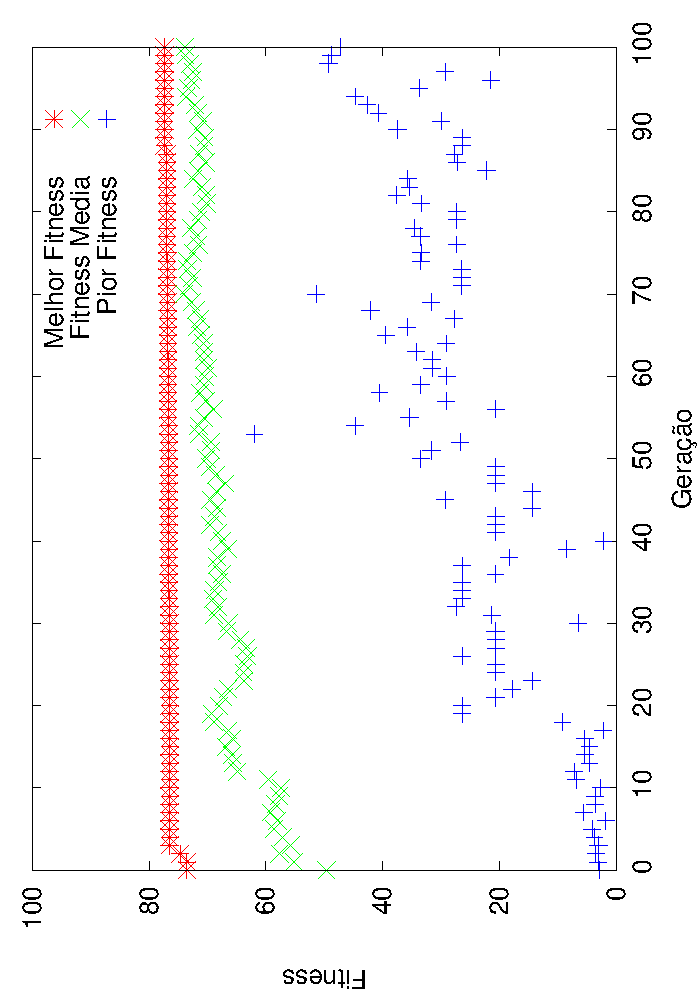
\includegraphics[angle=270, width=0.80\textwidth]{figures/acm.png}
 \caption{Variação da \textit{fitness} ao longo das gerações para a base da \textsc{ACM-DL}.}
\label{fig::fitnessgen}
\end{figure}

%%%%%%%%%%%%%%%%%%%%%%%%%%%%%%---------------------------------------------------%%%%%%%%%%%%%%%%%%%%%%%%%%%%%%
%%%%%%%%%%%%%%%%%%%%%%%%%%%%%%%---------------------------------------------------%%%%%%%%%%%%%%%%%%%%%%%%%%%%%%
%%%%%%%%%%%%%%%%%%%%%%%%%%%%%%%--------------        5.3          ----------------%%%%%%%%%%%%%%%%%%%%%%%%%%%%%%
%%%%%%%%%%%%%%%%%%%%%%%%%%%%%%%---------------------------------------------------%%%%%%%%%%%%%%%%%%%%%%%%%%%%%%
%%%%%%%%%%%%%%%%%%%%%%%%%%%%%%%---------------------------------------------------%%%%%%%%%%%%%%%%%%%%%%%%%%%%%%


\section{Metodologia Experimental}
\label{subsubsec::cv}

Para todos os experimentos, empregamos a técnica de Validação Cruzada (\cite{Refaeilzadeh00}) com 5 partições, com exceção dos testes na base de bioinformática, onde usamos 10 partições.
A validação cruzada é bem utilizada e aceita na literatura pelo seu poder se avaliação da generalização de um modelo. Ela consiste em dividir a base de dados em $k$ partições de tamanho igual, onde utilizamos $k-2$ para treinar um modelo, uma para a validação e uma para o teste final.
Combinamos a validação cruzada com nosso algoritmo de Programação Genética da seguinte forma: usamos o conjunto de treino para poder gerar o modelo de classificação, a validação para testar a \textit{fitness} dos indivíduos e reservamos o teste final para ser usado somente depois que já chegamos a um indivíduo evoluído.

Além disso, uma validação cruzada de $k$ partições dá origem a $k$ experimentos diferentes, onde cada um possui um conjunto diferente de treino, validação e testes, resultado da rotação das partições. A Figura~\ref{fig::cv} ilustra bem o processo de rotação para 5 partições, onde a partir de uma divisão inicial da base por 5 partições, podemos gerar os 5 experimentos mostrados.

\begin{figure}[h!]
  \centering
  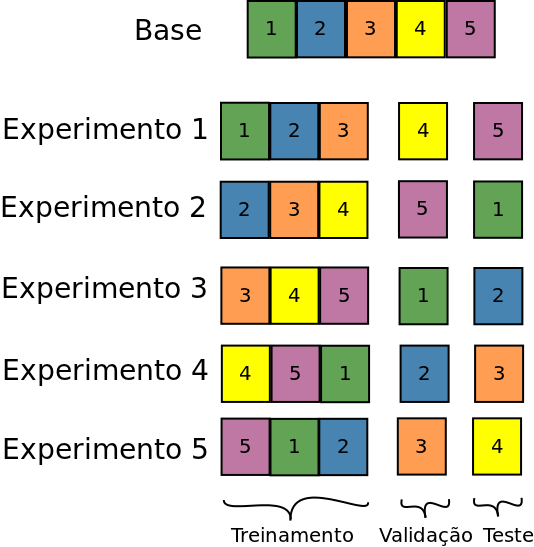
\includegraphics[width=0.40\textwidth]{figures/cv.png}
 \caption{Modelo de Validação Cruzada com 5 partições.}
\label{fig::cv}
\end{figure}

Como dito, pelo fato da base de bioinformática ser muito grande, tivemos que mudar a forma como os experimentos estavam sendo executados. Logo, ela foi dividida em 10 partições, sendo que usamos uma partição para treino, uma para validação e as outras 8 para teste. Dessa forma, evoluímos as funções de credibilidade em apenas dois décimos da base e utilizamos a função evoluída nos outros oito décimos.

Por fim, destacamos que todos os nossos resultados apresentados são analisados através do \textit{test-t} com nível de confiança de 99\%.

%%%%%%%%%%%%%%%%%%%%%%%%%%%%%%---------------------------------------------------%%%%%%%%%%%%%%%%%%%%%%%%%%%%%%
%%%%%%%%%%%%%%%%%%%%%%%%%%%%%%%---------------------------------------------------%%%%%%%%%%%%%%%%%%%%%%%%%%%%%%
%%%%%%%%%%%%%%%%%%%%%%%%%%%%%%%--------------        5.4          ----------------%%%%%%%%%%%%%%%%%%%%%%%%%%%%%%
%%%%%%%%%%%%%%%%%%%%%%%%%%%%%%%---------------------------------------------------%%%%%%%%%%%%%%%%%%%%%%%%%%%%%%
%%%%%%%%%%%%%%%%%%%%%%%%%%%%%%%---------------------------------------------------%%%%%%%%%%%%%%%%%%%%%%%%%%%%%%

\section{Credibilidade para Bases de Documentos}
\label{sec::documentos}

Nessa seção realizamos diferentes testes com as bases de documentos.
Iniciamos por mostrar na Seção~\ref{subsec::ganhosgp} como o uso de Programação Genética trouxe benefícios para que conseguíssemos obter funções de credibilidade mais eficazes. Esses
resultados que são válidos também para os demais experimentos mostrados nesse trabalho.
Já na Seção~\ref{subsec::generalidade} estudos os efeitos de aplicarmos uma função de credibilidade evoluída para uma determinada base em outras bases.
Por último, na Seção~\ref{subsec::fatores} trabalhamos com as redes de citação e autoria somadas aos atributos textuais, disponíveis somente para a base \textsc{ACM-DL}.

\subsection{Credibilidade de atributos}
\label{subsec::ganhosgp}

Na literatura, encontramos muitos trabalhos, conforme abordamos na Seção~\ref{sec::supervised}, que empregam várias das métricas de credibilidade de atributos utilizadas aqui, porém sem nenhuma combinação mais elaborada das mesmas.
Assim como previamente mencionamos na Seção~\ref{subsubsec::nbcredatributos} essas métricas sozinhas já poderiam ser funções de credibilidade de atributos, caso não usássemos o \textsc{PG}. Porém, não saberíamos dizer exatamente qual é a melhor métrica para usar em uma dada situação específica, e nem qual combinação, dentre as milhares existentes, é a melhor.

Com o intuito de mostrarmos que a combinação das métricas durante e evolução do \textsc{PG} é benéfica para a criação de uma função de credibilidade mais robusta e evitarmos a escolha de uma linha de base sem nenhuma informação adicional sobre as métricas, construímos as Tabelas~\ref{tab::imensamicro} e \ref{tab::imensamacro}.
Nelas, visualizamos a aplicação das diversas métricas de credibilidade nas quatro bases de texto que estudamos. Mostramos a linha de base na primeira linha, que trata do algoritmo \textit{Naïve Bayes} sem modificação, o \textsc{SVM} usado com o pacote \textit{SVMLight} (\cite{SVM}) na segunda linha, e as demais métricas nas outras linhas.
Entre parêntesis, temos a diferença da aplicação de uma métrica (ou \textsc{PG}) para a linha de base.
Vale ressaltar que utilizamos a função de \textit{kernel} linear para o \textsc{SVM}, que, como mostrado em \cite{Salles10}, é a melhor para quando temos uma alta dimensionalidade e tendência que as classes sejam linearmente separáveis, como acontece em bases de texto.

Vemos que usar o \textsc{PG} fornece uma solução bem mais robusta que usar qualquer um das outras métricas em separado. O resultado do \textsc{PG} da Micro$F_1$ da base \textsc{ACM-DL} foi o único que não trouxe resultados significativamente melhores, porém também não foram piores, como todas as outras métricas.
Observe que, nesse caso, o \textsc{PG} utilizou como terminais as trinta métricas para evolução dos atributos.

Os resultados com o \textsc{SVM} confirmam o que foi exibido em \cite{Salles10}, no qual o \textsc{SVM} apresenta resultados semelhantes aos do algoritmo \textit{Naïve Bayes}. É interessante destacar que nos cenários onde o \textsc{SVM} foi superior ao \textit{Naïve Bayes}, a utilização do \textsc{PG} fez com que essa diferença fosse nitidamente diminuída. Por exemplo, na Macro-$F_1$ da base \textit{Reuters}, onde os resultados do \textsc{SVM} não são estatisticamente superiores aos do \textsc{PG}.

Em geral, as métricas apresentaram resultados positivos em alguns cenários, mas negativos em outros, como a métrica \textsc{IDF} ou \textsc{GSS}. Mesmo as métricas que apresentaram resultados negativos em todos os experimentos, como \textsc{MaxTFIDF}, \textsc{MaxCTD}, foram mantidas como terminais para o algoritmo do \textsc{PG} por duas razões: (i) não temos certeza se existe um cenário no qual elas possam trazer benefícios, como usar uma outra base ou mesmo usar o inverso da métrica ($\frac{1}{MaxTFIDF}$), (ii) o \textsc{PG} naturalmente vai eliminar métricas que não trazem benefício ao longo das gerações.

Por fim, realizamos experimentos semelhantes para funções de credibilidade de relacionamentos na base da \textsc{ACM-DL}, obtendo o mesmo tipo de resultados que mostramos aqui, onde a função evoluída pelo \textsc{GP} é sempre melhor ou igual à aplicação das métricas em separado.


\begin{table}[h]
\centering
\caption{Avaliação da Micro$F_1$ com a aplicação de diversas métricas estudadas e o \textsc{PG}.}
\label{tab::imensamicro}
\begin{scriptsize}
\begin{adjustwidth}{-1cm}{-1cm}% adjust the L and R margins by 1 inch
\begin{tabular}{|c||c|c|c|c|}
%\begin{tabular*}{|c|c|c|c|c|}{@{\extracolsep{\fill}}lllr}

\toprule
\textbf{Métrica} & \textbf{ACM-DL} & \textbf{20ng} & \textbf{Ohsumed} & \textbf{Reuters}\tabularnewline
\midrule
\hline
Linha de Base & 73.63 \textpm{} 2.02 & 84.94 \textpm{} 0.58 & 66.56 \textpm{} 0.66 & 93.13 \textpm{} 0.29\tabularnewline
\hline 
\textbf{SVM} &
71.02 \textpm{} 0.77 &
80.03 \textpm{} 0.33 & 
70.39 \textpm{} 1.08 &
96.19 \textpm{} 0.33\tabularnewline
\hline 
\hline 
\rowcolor{LightCyan}
\textsc{PG} & 74.33 \textpm{} 0.72 (0.95 \ball) & 89.06 \textpm{} 0.15 (4.85 \triangOK) & 69.34 \textpm{} 0.55 (4.19 \triangOK) & 94.60 \textpm{} 0.44 (1.57 \triangOK)\tabularnewline
\hline 
TF(t) & 66.16 \textpm{} 5.91 (-10.14 \triangBAD) & 85.44 \textpm{} 0.69 (0.68 \ball) & 64.73 \textpm{} 3.16 (-2.74 \ball) & 86.32 \textpm{} 9.91 (-7.31 \ball)\tabularnewline
\hline 
TFClasse(t,c) & 66.93 \textpm{} 0.85 (-9.09 \triangBAD) & 86.74 \textpm{} 0.39 (2.21 \triangOK) & 67.06 \textpm{} 0.55 (0.76 \ball) & 92.80 \textpm{} 0.75 (-0.35 \ball)\tabularnewline
\hline 
DF(t) & 66.81 \textpm{} 0.64 (-9.26 \triangBAD) & 87.53 \textpm{} 0.28 (3.15 \triangOK) & 67.05 \textpm{} 0.71 (0.75 \ball) & 92.79 \textpm{} 0.77 (-0.37 \ball)\tabularnewline
\hline 
DFClasse(t,c) & 66.99 \textpm{} 0.82 (-9.02 \triangBAD) & 87.80 \textpm{} 0.31 (3.47 \triangOK) & 67.07 \textpm{} 0.55 (0.78 \ball) & 92.80 \textpm{} 0.75 (-0.35 \ball)\tabularnewline
\hline 
IDF(t) & 69.60 \textpm{} 0.79 (-5.47 \triangBAD) & 86.64 \textpm{} 0.43 (2.10 \triangOK) & 60.43 \textpm{} 0.72 (-9.21 \triangBAD) & 94.29 \textpm{} 0.35 (1.25 \triangOK)\tabularnewline
\hline 
IDFClasse(t,c) & 67.07 \textpm{} 0.77 (-8.91 \triangBAD) & 21.44 \textpm{} 32.33 (-74.73 \triangBAD) & 67.28 \textpm{} 0.42 (1.09 \triangOK) & 92.74 \textpm{} 0.46 (-0.42 \ball)\tabularnewline
\hline 
TFIDF(t,c) & 72.84 \textpm{} 1.05 (-1.06 \triangBAD) & 85.04 \textpm{} 0.30 (0.21 \ball) & 66.38 \textpm{} 0.70 (-0.27 \ball) & 93.77 \textpm{} 0.36 (0.68 \triangOK)\tabularnewline
\hline 
MaxTFIDF(t) & 65.40 \textpm{} 0.51 (-11.18 \triangBAD) & 81.25 \textpm{} 1.97 (-4.26 \triangBAD) & 62.56 \textpm{} 0.49 (-6.00 \triangBAD) & 87.60 \textpm{} 1.07 ( -5.94 \ball)\tabularnewline
\hline 
TFICF(t,c) & 58.75 \textpm{} 1.83 (-20.20 \triangBAD) & 84.99 \textpm{} 0.31 (0.16 \ball) & 60.43 \textpm{} 0.72 (-9.21 \triangBAD) & 72.41 \textpm{} 1.73 (-22.25 \triangBAD)\tabularnewline
\hline 
MaxTFICF(t) & 23.81 \textpm{} 1.29 (-67.66 \triangBAD) & 80.23 \textpm{} 1.62 (-5.45 \triangBAD) & 34.37 \textpm{} 0.40 (-48.35 \triangBAD) & 24.28 \textpm{} 1.02 (-73.93 \ball)\tabularnewline
\hline 
CTD(t,c) & 58.75 \textpm{} 1.83 (-20.20 \triangBAD) & 84.99 \textpm{} 0.31 (0.16 \ball) & 60.43 \textpm{} 0.72 (-9.21 \triangBAD) & 72.41 \textpm{} 1.73 (-22.25 \triangBAD)\tabularnewline
\hline 
MaxCTD(t) & 37.69 \textpm{} 2.08 (-48.81 \triangBAD) & 80.14 \textpm{} 0.45 (-5.56 \triangBAD) & 48.34 \textpm{} 0.80 (-27.36 \triangBAD) & 61.78 \textpm{} 1.59 (-33.67 \triangBAD)\tabularnewline
\hline 
DOM(t,c) & 73.38 \textpm{} 0.97 (-0.33 \triangBAD) & 84.65 \textpm{} 0.37 (-0.24 \ball) & 64.15 \textpm{} 0.59 (-3.62 \triangBAD) & 93.43 \textpm{} 0.38 (0.31 \ball)\tabularnewline
\hline 
MaxDom(t) & 72.25 \textpm{} 0.70 (-1.87 \triangBAD) & 85.66 \textpm{} 0.31 (0.94 \triangOK) & 67.99 \textpm{} 0.58 (2.15 \triangOK) & 92.73 \textpm{} 0.64 (-0.43 \ball)\tabularnewline
\hline 
AM(t,c) & 73.13 \textpm{} 1.05 (-0.68 \triangBAD) & 81.98 \textpm{} 0.48 (-1.96 \triangBAD) & 64.21 \textpm{} 0.60 (-3.52 \triangBAD) & 93.43 \textpm{} 0.38 (0.31 \ball)\tabularnewline
\hline 
MaxAM(t) & 72.17 \textpm{} 0.67 (-1.97 \triangBAD) & 85.36 \textpm{} 0.18 (0.59 \ball) & 67.97 \textpm{} 0.61 (2.12 \triangOK) & 92.73 \textpm{} 0.64 (-0.43 \ball)\tabularnewline
\hline 
P(t|c) & 72.96 \textpm{} 1.06 (-0.90 \triangBAD) & 84.93 \textpm{} 1.32 (0.08 \ball) & 63.33 \textpm{} 1.09 (-4.84 \triangBAD) & 93.32 \textpm{} 0.38 (0.20 \ball)\tabularnewline
\hline 
P($\overline{t}$|c) & 63.43 \textpm{} 0.90 (-13.85 \triangBAD) & 86.22 \textpm{} 0.29 (1.60 \triangOK) & 62.51 \textpm{} 0.79 (-6.08 \triangBAD) & 92.84 \textpm{} 0.43 (-0.32 \ball)\tabularnewline
\hline 
%\rowcolor{LightCyan}
GINI(t) & 71.35 \textpm{} 0.77 (-3.10 \triangBAD) & 84.81 \textpm{} 0.15 (-0.06 \ball) & 68.82 \textpm{} 0.47 (3.41 \triangOK) & 92.45 \textpm{} 0.60 (-0.73 \ball) \tabularnewline
\hline 
IG(t,c) & 71.31 \textpm{} 0.65 (-3.15 \triangBAD) & 86.85 \textpm{} 0.34 (2.34 \triangOK) & 68.18 \textpm{} 0.58 (2.45 \triangOK) & 94.04 \textpm{} 0.46 (0.97 \triangOK)\tabularnewline
\hline 
MaxIG(t) & 68.49 \textpm{} 0.60 (-6.98 \triangBAD) & 87.62 \textpm{} 0.34 (3.25 \triangOK) & 67.74 \textpm{} 0.66 (1.77 \triangOK) & 93.61 \textpm{} 0.70 (0.51 \ball)\tabularnewline
\hline 
CE(t) & 44.65 \textpm{} 0.34 (-39.35 \triangBAD) & 54.16 \textpm{} 1.48 (-36.17 \triangBAD) & 31.86 \textpm{} 0.13 (-52.13 \triangBAD) & 76.72 \textpm{} 0.44 (-17.67 \triangBAD)\tabularnewline
\hline 
CHI(t,c) & 69.86 \textpm{} 0.74 (-5.12 \triangBAD) & 87.23 \textpm{} 0.39 (2.79 \triangOK) & 67.99 \textpm{} 0.54 (2.16 \triangOK) & 93.76 \textpm{} 0.54 (0.67 \triangOK)\tabularnewline
\hline 
MaxCHI(t) & 68.41 \textpm{} 0.58 (-7.09 \triangBAD) & 87.55 \textpm{} 0.29 (3.17 \triangOK) & 67.35 \textpm{} 0.64 (1.19 \triangOK) & 93.22 \textpm{} 0.81 (0.09 \ball)\tabularnewline
\hline 
CC(t,c) & 69.69 \textpm{} 0.70 (-5.35 \triangBAD) & 72.19 \textpm{} 7.43 (-14.93 \triangBAD) & 67.96 \textpm{} 0.54 (2.11 \triangOK) & 93.58 \textpm{} 0.55 (0.66 \ball)\tabularnewline
\hline 
MaxCC(t) & 1.49 \textpm{} 0.05 (-97.98 \triangBAD) & 5.29 \textpm{} 0.02 (-93.77 \triangBAD) & 7.26 \textpm{} 0.01 (-89.10 \triangBAD) & 5.22 \textpm{} 0.05 (-94.40 \triangBAD)\tabularnewline
\hline 
GSS(t,c) & 69.65 \textpm{} 0.71 (-5.40 \triangBAD) & 72.19 \textpm{} 7.43 (-14.93 \triangBAD) & 67.95 \textpm{} 0.56 (2.10 \triangOK) & 93.77 \textpm{} 0.54 (0.68 \triangOK)\tabularnewline
\hline 
MaxGSS(t) & 1.48 \textpm{} 0.06 (-97.99 \triangBAD) & 5.29 \textpm{} 0.02 (-93.77 \triangBAD) & 7.26 \textpm{} 0.01 (-89.10 \triangBAD) & 5.19 \textpm{} 0.04 (-94.42 \triangBAD)\tabularnewline
\hline 
OR(t,c) & 68.54 \textpm{} 0.95 (-6.91 \triangBAD) & 84.77 \textpm{} 0.19 (-0.11 \ball) & 65.59 \textpm{} 0.84 (-1.45 \ball) & 92.42 \textpm{} 0.59 (-0.76 \triangBAD)\tabularnewline
\hline 
MaxOR(t) & 48.15 \textpm{} 0.43 (-34.60 \triangBAD) & 65.20 \textpm{} 0.71 (-23.17 \triangBAD) & 34.75 \textpm{} 0.14 (-47.79 \triangBAD) & 79.99 \textpm{} 0.27 (-14.12 \triangBAD)\tabularnewline
\bottomrule
\end{tabular}
\end{adjustwidth}
\end{scriptsize}
\end{table}

%\noindent\makebox[\textwidth]{%
%\begin{tabularx}{1.5\textwidth}{XX}


\begin{table}[h]
%\centering
\caption{Avaliação da Macro$F_1$ com a aplicação de diversas métricas estudadas e o \textsc{PG}.}
\label{tab::imensamacro}
\begin{scriptsize}
\begin{adjustwidth}{-1cm}{-1cm}% adjust the L and R margins by 1 inch
\begin{tabular}{|c||c|c|c|c|}
\toprule
\textbf{Métricas} & \textbf{ACM-DL}& \textbf{20ng}& \textbf{Ohsumed}& \textbf{Reuters}\tabularnewline
\midrule
\hline
Linha de Base& 57.26 \textpm{} 2.08& 83.68 \textpm{} 0.82& 54.76 \textpm{} 1.27& 81.96 \textpm{} 1.44\tabularnewline
\hline 
\textbf{SVM} & 59.44 \textpm{} 0.44 & 79.83 \textpm{} 0.33 &
64.72 \textpm{} 1.51 & 
91.92 \textpm{} 1.21\tabularnewline
\hline 
\rowcolor{LightCyan}
\textsc{PG}& 59.72 \textpm{} 1.26 (4.30 \triangOK)& 88.69 \textpm{} 0.22 (5.99 \triangOK)& 63.56 \textpm{} 0.89 (16.06 \triangOK)& 89.33 \textpm{} 0.90 (8.99 \triangOK)\tabularnewline
\hline 
TF(t)& 54.89 \textpm{} 3.33 (-4.14 \ball)& 83.12 \textpm{} 2.08 (-0.59 \ball)& 58.48 \textpm{} 2.76 (6.80 \triangOK)& 79.64 \textpm{} 9.43 (-2.83 \ball)\tabularnewline
\hline 
TFClasse(t,c)& 55.57 \textpm{} 0.72 (-2.95 \triangBAD)& 85.66 \textpm{} 0.55 (2.44 \triangOK)& 61.66 \textpm{} 1.36 (12.59 \triangOK)& 87.56 \textpm{} 1.55 (6.84 \triangOK)\tabularnewline
\hline 
DF(t)& 55.83 \textpm{} 0.57 (-2.50 \triangBAD)& 86.85 \textpm{} 0.39 (3.86 \triangOK)& 61.43 \textpm{} 1.49 (12.18 \triangOK)& 87.24 \textpm{} 0.98 (6.44 \triangOK)\tabularnewline
\hline 
DFClasse(t,c)& 55.60 \textpm{} 0.70 (-2.89 \triangBAD) & 87.22 \textpm{} 0.38 (4.30 \triangOK)& 61.71 \textpm{} 1.41 (12.69 \triangOK)& 87.56 \textpm{} 1.55 (6.84 \triangOK) \tabularnewline
\hline 
IDF(t) & 56.84 \textpm{} 0.80 (-0.73 \triangBAD) & 85.58 \textpm{} 0.57 (2.35 \triangOK) & 57.07 \textpm{} 0.52 (4.22 \triangOK) & 89.01 \textpm{} 0.60 (8.61 \triangOK)\tabularnewline
\hline 
IDFClasse(t,c) & 54.88 \textpm{} 0.61 (-4.15 \triangBAD) & 17.43 \textpm{} 33.83 (-79.16 \triangBAD) & 61.50 \textpm{} 1.36 (12.31 \triangOK) & 85.94 \textpm{} 0.85 (4.86 \triangOK) \tabularnewline
\hline 
TFIDF(t,c)& 58.33 \textpm{} 1.08 (1.87 \triangOK)& 83.85 \textpm{} 0.40 (0.28 \ball)& 56.37 \textpm{} 1.29 (2.94 \triangOK)& 85.25 \textpm{} 0.64 (4.01 \triangOK)\tabularnewline
\hline 
MaxTFIDF(t)& 54.33 \textpm{} 0.41 (-5.12 \triangBAD)& 80.24 \textpm{} 1.51 (-4.05 \triangBAD)& 59.62 \textpm{} 1.14 (8.87 \triangOK)& 82.65 \textpm{} 1.74 (0.84 \ball)\tabularnewline
\hline 
TFICF(t,c)& 50.63 \textpm{} 0.97 (-11.58 \triangBAD)& 80.60 \textpm{} 1.52 (-3.61 \triangBAD)& 57.07 \textpm{} 0.52 (4.22 \triangOK)& 66.44 \textpm{} 1.50 (-18.93 \triangBAD)\tabularnewline
\hline 
MaxTFICF(t)& 28.94 \textpm{} 0.93 (-49.46 \triangBAD)& 76.26 \textpm{} 0.18 (-8.81 \triangBAD)& 38.85 \textpm{} 0.88 (-29.05 \triangBAD)& 32.38 \textpm{} 1.54 (-60.49 \ball)\tabularnewline
\hline 
CTD(t,c)& 50.63 \textpm{} 0.97 (-11.58 \triangBAD)& 80.60 \textpm{} 1.52 (-3.61 \triangBAD)& 57.07 \textpm{} 0.52 (4.22 \triangOK)& 66.44 \textpm{} 1.50 (-18.93 \triangBAD)\tabularnewline
\hline 
MaxCTD(t)& 38.29 \textpm{} 1.43 (-33.13 \triangBAD)& 77.38 \textpm{} 1.13 (-7.47 \triangBAD)& 48.40 \textpm{} 0.94 (-11.62 \triangBAD)& 54.09 \textpm{} 0.96 (-34.01 \triangBAD)\tabularnewline
\hline 
DOM(t,c)& 58.34 \textpm{} 1.62 (1.89 \ball)&  83.21 \textpm{} 0.55 (-0.49 \triangBAD)& 51.77 \textpm{} 1.00 (-5.47 \triangBAD)& 85.28 \textpm{} 0.87 (4.06 \triangOK)\tabularnewline
\hline 
MaxDom(t)& 58.74 \textpm{} 1.27 (2.58 \triangOK)& 84.31 \textpm{} 0.52 (0.82 \ball)& 62.60 \textpm{} 0.83 (14.32 \triangOK)& 87.07 \textpm{} 0.95 (6.23 \triangOK)\tabularnewline
\hline 
AM(t,c)& 58.02 \textpm{} 1.73 (1.33 \ball)& 83.78 \textpm{} 0.27 (-1.27 \triangBAD) & 52.21 \textpm{} 1.12 (-4.65 \triangBAD)& 85.28 \textpm{} 0.87 (4.06 \triangOK)\tabularnewline
\hline 
MaxAM(t)& 58.64 \textpm{} 1.20 (2.41 \triangOK)& 83.68 \textpm{} 0.27 (0.07 \ball)& 62.93 \textpm{} 1.03 (14.91 \triangOK)& 87.07 \textpm{} 0.95 (6.23 \triangOK)\tabularnewline
\hline 
P(t|c)& 57.51 \textpm{} 1.54 (0.44 \ball)& 82.62 \textpm{} 1.55 (-1.20 \ball)& 54.20 \textpm{} 2.53 (-1.02 \ball)& 84.92 \textpm{} 0.81 (3.61 \triangOK)\tabularnewline
\hline 
P($\overline{t}$|c)& 52.25 \textpm{} 0.90 (-8.75 \triangBAD)& 83.42 \textpm{} 1.83 (-0.24 \ball)& 56.36 \textpm{} 1.39 (2.92 \triangOK)& 87.42 \textpm{} 0.40 (6.66 \triangOK)\tabularnewline
\hline 
%\rowcolor{LightCyan}
GINI(t)& 58.11 \textpm{} 1.00 (1.49 \triangOK)& 83.10 \textpm{} 0.25 (-0.62 \ball)& 63.29 \textpm{} 1.25 (15.58 \triangOK)& 86.58 \textpm{} 0.95 (5.63 \triangOK)\tabularnewline
\hline 
IG(t,c)& 58.06 \textpm{} 1.04 (1.41 \triangOK)& 85.89 \textpm{} 0.43 (2.71 \triangOK)& 62.91 \textpm{} 1.44 (14.89 \triangOK)& 88.88 \textpm{} 0.93 (8.44 \triangOK)\tabularnewline
\hline 
MaxIG(t)& 56.42 \textpm{} 0.63 (-1.47 \ball)& 87.07 \textpm{} 0.34 (4.12 \triangOK)& 62.24 \textpm{} 1.53 (13.66 \triangOK)& 88.05 \textpm{} 1.01 (7.43 \triangOK)\tabularnewline
\hline 
CE(t)& 22.94 \textpm{} 0.41 (-59.93 \triangBAD)&  50.23 \textpm{} 1.40 (-39.93 \triangBAD)& 8.78 \textpm{} 0.11 (-83.96 \triangBAD)& 31.55 \textpm{} 1.48 (-61.73 \triangBAD)\tabularnewline
\hline 
CHI(t,c)& 56.81 \textpm{} 1.00 (-0.78 \ball)& 86.54 \textpm{} 0.46 (3.49 \triangOK)& 62.59 \textpm{} 1.41 (14.30 \triangOK)& 88.31 \textpm{} 0.95 (7.75 \triangOK)\tabularnewline
\hline 
MaxCHI(t)& 56.22 \textpm{} 0.64 (-1.8 \triangBAD)& 87.01 \textpm{} 0.34 (4.05 \triangOK)& 61.67 \textpm{} 1.50 (12.61 \triangOK)& 87.43 \textpm{} 1.22 (6.68 \triangOK)\tabularnewline
\hline 
CC(t,c)& 56.93 \textpm{} 0.90 (-0.57 \ball)&  74.52 \textpm{} 5.89 (-10.89 \triangBAD)& 62.57 \textpm{} 1.37 (14.25 \triangOK)& 88.56 \textpm{} 0.02 (7.31 \triangOK) \tabularnewline
\hline 
MaxCC(t)& 0.27 \textpm{} 0.01 (-99.52 \triangBAD)& 0.53 \textpm{} 0.02 (-99.36 \triangBAD)& 0.59 \textpm{} 0.00 (-98.93 \triangBAD)& 1.32 \textpm{} 0.18 (-98.39 \triangBAD)\tabularnewline
\hline 
GSS(t,c)& 56.90 \textpm{} 0.91 (-0.62 \ball)& 74.52 \textpm{} 5.89 (-10.89 \triangBAD)& 62.57 \textpm{} 1.39 (14.25 \triangOK)& 88.43 \textpm{} 0.91 (7.90 \triangOK)\tabularnewline
\hline 
MaxGSS(t)& 0.26 \textpm{} 0.01 (-99.54 \triangBAD)& 0.53 \textpm{} 0.02 (-99.36 \triangBAD)& 0.59 \textpm{} 0.00 (-98.93 \triangBAD)& 1.23 \textpm{} 0.01 (-98.49 \triangBAD)\tabularnewline
\hline 
OR(t,c)& 56.80 \textpm{} 1.22 (-0.80 \ball)& 83.20 \textpm{} 0.39 (-0.51 \ball)& 60.67 \textpm{} 1.55 (10.79 \triangOK)& 86.67 \textpm{} 0.56 (5.75 \triangOK)\tabularnewline
\hline
MaxOR(t)& 28.15 \textpm{} 0.74 (-50.83 \triangBAD)& 62.09 \textpm{} 0.51 (-25.75 \triangBAD)& 12.21 \textpm{} 0.28 (-77.70 \triangBAD)& 40.94 \textpm{} 1.06 (-50.04 \triangBAD)\tabularnewline
\bottomrule
\end{tabular}
\end{adjustwidth}
\end{scriptsize}
\end{table}

%\end{tabularx}}



%%%%%%%%%%%%%%%%%%-------%%%%%%%%%%%%%%%
%%%%%%%%%%%%%%%%%%-------%%%%%%%%%%%%%%%

\subsection{Generalidade}
\label{subsec::generalidade}

Na Seção~\ref{subsec::ganhosgp}, analisamos os resultados obtidos ao aplicar todas as métricas de credibilidade de atributos em separado e através do uso de \textsc{PG}.
Como mencionamos na Seção~\ref{subsubsec::cv}, usamos validação cruzada com 5 partições para o obter os resultados mostrados na Tabelas~\ref{tab::imensamicro} e \ref{tab::imensamacro}.
Logo, para cada uma das bases, tivemos cinco funções evoluídas pelo uso do \textsc{PG}, uma para cada rotação, como mostrado na Figura~\ref{fig::cv}.
Cada uma dessas funções obteve um resultado em seu experimento e exibimos, ao final, os resultados médios das cinco funções e desvio padrão.
Decidimos por escolher a função que obteve o melhor resultado em seu experimento como representante da base de dados e mostramos essas funções na Tabela~\ref{tab::representantes}.
Assim, por exemplo, a $F_{ACM-DL}$ mostrada foi a função escolhida para a base \textsc{ACM-DL} por ter obtido maiores ganhos que as outras quatro funções evoluídas.

\begin{table}[!h]
\renewcommand{\arraystretch}{1.3}
\centering
\caption{Funções de credibilidade geradas para cada uma das bases.}
\label{tab::representantes}
\begin{scriptsize}
\begin{tabular}{|c||c|}
\toprule
\textbf{Base} & \textbf{Função de Credibilidade}\tabularnewline
\midrule
\hline
ACM-DL   & $F_{ACM-DL} =  DOM^{(GSS)^{(CE + TF)}} $\tabularnewline
\hline
20ng & $F_{20ng} = DF + MaxAM + (\dfrac{ CHI } { TFIDF^{(MaxTFIDF)} }) $\tabularnewline
\hline
Ohsumed  & $ F_{Ohsumed} = (\dfrac{AM}{MaxIG \times CC^{(sumDF)}} )^{(TFICF)^{(TFICF)}} $\tabularnewline
\hline
Reuters & $ F_{Reuters} = IG^{(MaxIG \times GINI)}$\tabularnewline
\bottomrule
\end{tabular}
\end{scriptsize}
\end{table}

Resolvemos então aplicar as melhores funções evoluídas para cada base nas demais bases (e nos outros experimentos de uma mesma base também). Assim podemos testar o quanto uma função de credibilidade evoluída para uma determinada base é geral e pode ser usada em outro contexto. Nas Tabelas~\ref{tab::generalizacao-Micro} e \ref{tab::generalizacao-Macro}, observamos os resultados do estudo da generalização das funções. Se analisarmos as tabelas na linha diagonal central, veremos a aplicação das funções da Tabela~\ref{tab::representantes} em toda a base, não mais em apenas um dos cinco experimentos da validação cruzada. Observe que todos os resultados são tão bons ou melhores que os reportados anteriormente na Seção~\ref{subsec::ganhosgp}. Em especial, esse foi o único resultado que apresentou ganhos significativos para base da \textsc{ACM-DL}.

Ao observarmos as Tabelas~\ref{tab::generalizacao-Micro} e \ref{tab::generalizacao-Macro} coluna a coluna, vemos o comportamento de cada uma das funções em cada uma das bases. É nítido que nenhuma das funções evoluídas nas outras bases foi boa para a base da \textsc{ACM-DL}, e nem a função evoluída pela \textsc{ACM-DL} obteve resultados bons para as outras bases.
Acreditamos que isso é devido ao fato da proximidade existente entre as classes que pertencem à base da \textsc{ACM-DL}, i. e., enquanto as outras bases apresentam grandes diferenças semânticas entre as diversas classes, a base da \textsc{ACM-DL} apresenta classes muito mais semelhantes e, portanto, mais difíceis de serem separadas. Por isso, existe uma dificuldade maior em encontrar uma função que capture melhor esse fato e, assim, a base da \textsc{ACM-DL} não generaliza bem.
Verificamos também, através das tabelas, que todas funções tiveram êxito na melhora da Macro$F_1$ das bases \textit{Ohsumed} e \textit{Reuters}, mas o mesmo não ocorreu na Micro$F_1$.
Finalmente, destacamos que a única função que obteve resultados bons nas demais bases (exceto na Micro$F_1$ da \textsc{ACM}) foi a função evoluída para a base \textit{20ng}.
Sendo assim, concluímos que usar as funções evoluídas pelo \textsc{PG} se comportam muito bem na própria base, mas não podemos dizer o mesmo para as demais bases.

Por fim, uma análise interessante pode ser feita usando as funções mostradas na Tabela~\ref{tab::representantes} e verificando os resultados obtidos por utilizar cada uma delas individualmente como feito nas Tabelas~\ref{tab::imensamicro} e~\ref{tab::imensamacro}. Por exemplo para a base \textsc{ACM-DL}, as métricas \textsc{DOM}, \textsc{GSS}, \textsc{CE} e \textsc{TF} foram combinadas usando as operações de potência e soma resultado em um ganho estatisticamente significativo de 1.91\% para a Micro$F_1$, enquanto essas métricas isoladas obtiveram perdas significativas em relação à linha de base, com um máximo de -39.35\% da métrica \textsc{CE}.


\begin{table}[!h]
\centering
\caption{Micro$F_1$ obtida pelo \textit{Naïve Bayes} quando usando a função de credibilidade $F_{base}$ gerada uma dada base nas demais bases.}
\label{tab::generalizacao-Micro}
\begin{scriptsize}
\begin{adjustwidth}{-1cm}{-1cm}% adjust the L and R margins by 1 inch
\begin{tabular}{|c|c|c|c|c|}
\toprule
 & \textbf{ACM-DL} & \textbf{20ng} & \textbf{Ohsumed} & \textbf{Reuters}\tabularnewline
\midrule
\hline
Linha de Base & 73.63 \textpm{} 0.90 & 84.86 \textpm{} 0.54 & 66.56 \textpm{} 0.66 & 93.13 \textpm{} 0.29\tabularnewline
\hline
$F_{ACM-DL}$ & 75.04 \textpm{} 0.88 (1.91 \triangOK) & 84.45 \textpm{} 0.35 (-0.49 \triangBAD) & 66.06 \textpm{} 0.59 (-0.75 \ball) & 92.68 \textpm{} 0.45 (-0.48 \triangBAD)\tabularnewline
\hline
$F_{20ng}$ & 66.69 \textpm{} 0.65 (-9.42 \triangBAD) & 88.97 \textpm{} 0.17 (4.84 \triangOK) & 67.94 \textpm{} 0.62 (2.08 \triangOK)  & 94.01 \textpm{} 0.53 (0.94 \triangOK)\tabularnewline
\hline
$F_{Ohsumed}$ & 70.09 \textpm{} 0.82 (-4.81 \triangBAD) & 85.60 \textpm{} 0.27 (0.87 \triangOK) & 69.54 \textpm{} 0.69 (4.49 \triangOK) & 93.45 \textpm{} 0.57 (0.34 \ball)\tabularnewline
\hline
$F_{Reuters}$ & 66.55 \textpm{} 0.89 (-9.61 \triangBAD) & 87.04 \textpm{} 0.41 (2.57 \triangOK) & 63.32 \textpm{} 0.82 (-4.86 \triangBAD) & 94.87 \textpm{} 0.25 (1.86 \triangOK)\tabularnewline
\bottomrule
\end{tabular}
\end{adjustwidth}
\end{scriptsize}
\end{table}


\begin{table}[!h]
\centering
\caption{Macro$F_1$ obtida pelo \textit{Naïve Bayes} quando usando a função de credibilidade $F_{base}$ gerada uma dada base nas demais bases.}
\label{tab::generalizacao-Macro}
\begin{scriptsize}
\begin{adjustwidth}{-1cm}{-1cm}% adjust the L and R margins by 1 inch
\begin{tabular}{|c|c|c|c|c|}
\toprule
 & \textbf{ACM-DL} & \textbf{20ng} & \textbf{Ohsumed} & \textbf{Reuters}\tabularnewline
\midrule
\hline
Linha de Base & 57.26 \textpm{} 0.93 & 83.62 \textpm{} 0.74 & 54.76 \textpm{} 1.27 & 81.96 \textpm{} 1.44\tabularnewline
\hline
$F_{ACM-DL}$ & 60.13 \textpm{} 1.44 (5.02 \triangOK) & 82.88 \textpm{} 0.51 (-0.89 \triangBAD) & 56.41 \textpm{}  0.92 (3.00 \triangOK) & 85.49 \textpm{} 0.94 (4.31 \triangOK)\tabularnewline
\hline
$F_{20ng}$ & 55.83 \textpm{} 0.66 (-2.50 \triangBAD) & 88.63 \textpm{} 0.18 (5.99 \triangOK) & 62.12 \textpm{} 1.41 (13.43 \triangOK) & 88.64 \textpm{} 1.03 (8.16 \triangOK)\tabularnewline
\hline
$F_{Ohsumed}$ & 57.59 \textpm{} 0.56 (0.58 \ball) & 84.26 \textpm{}  0.49 (0.77 \triangOK) & 64.35 \textpm{} 1.17 (17.51 \triangOK) & 87.41 \textpm{} 0.64 (6.65 \triangOK)\tabularnewline
\hline
$F_{Reuters}$ & 54.84 \textpm{} 1.44 (-4.23 \triangBAD) & 83.15 \textpm{} 2.04 (-0.56 \ball) & 57.97 \textpm{} 1.59 (5.85 \triangOK) & 89.45 \textpm{}  0.74 (9.14 \triangOK)\tabularnewline
\bottomrule
\end{tabular}
\end{adjustwidth}
\end{scriptsize}
\end{table}

%%%%%%%%%%%%%%%%%%-------%%%%%%%%%%%%%%%
%%%%%%%%%%%%%%%%%%-------%%%%%%%%%%%%%%%

\subsection{Explorando Relacionamentos e Múltiplos Fatores}
\label{subsec::fatores}

Nessa seção avaliamos como o uso de mais de um fator pode tornar o cálculo da credibilidade mais preciso. Somente a base da \textsc{ACM} apresenta informações disponíveis sobre os autores e as citações contidas em seus documentos. Portanto, essa foi a única base que pudemos realizar experimentos com mais de um fator.

Na Tabela~\ref{tab::fatores}, mostramos a aplicação dos fatores isoladamente e a combinação dos mesmos. A primeira coluna, termos, se refere a credibilidade dos atributos e as segunda e terceira colunas, à credibilidade dos relacionamentos. Vemos que simplesmente usar a rede de autoria ou citações provê benefícios imediatos que não foram alcançados ao explorarmos os atributos.

Esse fato evidencia o poder da classificação relacional, e que podemos obter ganhos acentuados ao explorar a credibilidade dos relacionamentos. Com única exceção da Micro$F_1$ ao aplicar os três fatores, observamos que quanto mais fatores envolvemos na credibilidade, melhores são os resultados. Por exemplo, ao usar somente a citação, temos ganhos de 3.4\% na Micro$F_1$ e 5.43\% na Macro$F_1$, ao combinar a citação com os termos, os ganhos vão para 4.18\% e 7.96\%. Acreditamos que não obtemos um resultado ainda mais expressivo para a combinação dos três fatores pelo fato que o número de métricas é muito elevado (30 dos atributos e 16 para cada um dos relacionamentos) e os parâmetros usados no \textsc{PG} não foram otimizados para esse caso.


\begin{table}[!h]
\centering
\caption{Resultados do uso de credibilidade na base da \textsc{ACM-DL} explorando a credibilidade de termos, autoria e citação.}
\label{tab::fatores}
\begin{footnotesize}
\begin{tabular}{|c|c|c||c|c|}
\toprule
\multicolumn{3}{|c||}{\textbf{Fatores}} & \multirow{2}{*}{\textbf{Micro$F_1$}} & \multirow{2}{*}{\textbf{Macro$F_1$}} \tabularnewline \cline{1-3}
\textbf{Termos} & \textbf{Autoria} & \textbf{Citação} & & \multicolumn{1}{c|}{}  \tabularnewline % & \textbf{Micro$F_1$} & \textbf{Macro$F_1$}\tabularnewline
\midrule
\hline
\multicolumn{3}{|c||}{Linha de Base} & 73.63 \textpm{} 0.91 & 57.26 \textpm{} 0.93\tabularnewline
\hline
X &  &  & 74.33 \textpm{} 0.72 (0.95 \ball) & 59.72 \textpm{} 1.26 (4.30 \triangOK)\tabularnewline
\hline
 & X &  & 76.19 \textpm{} 0.82 (3.48 \triangOK) & 60.37 \textpm{} 0.70 (5.43 \triangOK)\tabularnewline
\hline
 &  & X & 75.58 \textpm{} 0.85 (2.65 \triangOK) & 59.00 \textpm{} 0.90 (3.04 \triangOK)\tabularnewline
\hline
X & X &  & 76.70 \textpm{} 1.08 (4.18 \triangOK) & 61.82 \textpm{} 1.38 (7.96 \triangOK)\tabularnewline
\hline
X &  & X & 75.63 \textpm{} 1.03 (2.72 \triangOK) & 60.69 \textpm{} 1.30 (5.98 \triangOK)\tabularnewline
\hline
 & X & X & 77.29 \textpm{} 0.79 (4.98 \triangOK) & 61.41 \textpm{} 0.65 (7.25 \triangOK)\tabularnewline
\hline
X & X & X & 77.01 \textpm{} 0.98 (4.60 \triangOK) & 62.24 \textpm{} 1.01 (8.70 \triangOK)\tabularnewline
\bottomrule
\end{tabular}
\end{footnotesize}
\end{table}

%%%%%%%%%%%%%%%%%%-------%%%%%%%%%%%%%%%
%%%%%%%%%%%%%%%%%%-------%%%%%%%%%%%%%%%
%%%%%%%%%%%%%%%%%%-------%%%%%%%%%%%%%%%

%%%%%%%%%%%%%%%%%%%%%%%%%%%%%%---------------------------------------------------%%%%%%%%%%%%%%%%%%%%%%%%%%%%%%
%%%%%%%%%%%%%%%%%%%%%%%%%%%%%%%---------------------------------------------------%%%%%%%%%%%%%%%%%%%%%%%%%%%%%%
%%%%%%%%%%%%%%%%%%%%%%%%%%%%%%%--------------        5.5          ----------------%%%%%%%%%%%%%%%%%%%%%%%%%%%%%%
%%%%%%%%%%%%%%%%%%%%%%%%%%%%%%%---------------------------------------------------%%%%%%%%%%%%%%%%%%%%%%%%%%%%%%
%%%%%%%%%%%%%%%%%%%%%%%%%%%%%%%---------------------------------------------------%%%%%%%%%%%%%%%%%%%%%%%%%%%%%%


\section{Credibilidade em Bases de Atributos Categóricos}
\label{sec::categorias}


Na Seção~\ref{sec::supervised}, vimos que vários trabalhos lidam com o uso de diversas das métricas que utilizamos para gerar funções de credibilidade de atributos. Um ponto comum a todos
é que se preocupam somente com classificação de documentos, ou seja, os atributos são sempre textuais. Expandimos essa abordagem ao lidar também com atributos categóricos.

Nas Tabelas~\ref{tab::cat-micro} e \ref{tab::cat-macro}, mostramos os resultados de evoluir funções de credibilidade para as bases usando tanto o algoritmo de classificação \textit{Naïve Bayes} quanto o \textsc{KNN}. Dessa vez, mostramos os resultados com o \textsc{KNN} pelo fato de sua linha de base ser muito superior à do \textit{Naïve Bayes} (excepto para a Micro$F_1$ da base \textit{Nursery}). A título de informação, utilizamos $K$ = 6, 9, 10, 8 para as bases \textit{Cars}, \textit{Tictac}, \textit{Nursery} e \textit{Chess}, respectivamente. Esses valores foram definidos em experimentos preliminares.

Destacamos os ganhos mais interessantes na Macro$F_1$ da base \textit{Cars}. Esse fato evidencia que os exemplos de maior dificuldade, por serem de classes menos populares, foram corretamente classificados. Isso alterou muito pouco a Micro$F_1$, pois, em quantidade, os exemplos difíceis são poucos, mas alterou muito a Macro$F_1$, pois existiram aumentos substanciais na métrica $F_1$ das classes com menos exemplos. O mesmo ocorre na base \textit{Nursery} quando usamos o \textit{Naïve Bayes}. Já as bases \textit{TicTacToe} e \textit{Chess} apresentaram ganhos pequenos, inferiores a 2\%.
%(talvez mostrando que funções de crediblidade nao sao boas para jogos!)

Uma análise das funções evoluídas em todas as bases (não mostramos as funções pelo fato delas serem 40 distintas (5 por base, 4 bases, 2 algoritmos)), mostra que as métricas \textsc{AM}, \textsc{CHI}, \textsc{Gini} e \textsc{IG} são as mais frequentes, sendo que ao menos uma delas aparece em todas as funções. Por outro lado, as métricas que calculam máximos, \textsc{MaxAM}, \textsc{MaxCC}, entre outras, não apareceram. Isso pode mostrar que métricas globais são menos efetivas para métrica de credibilidade de atributos categóricos.

%COM SVM
%\begin{table}[h!]
%\centering
%\caption{Resultados da Micro$F_1$ para as bases de atributos categóricos}
%\label{tab::cat-micro}
%\begin{footnotesize}
%\begin{adjustwidth}{-1cm}{-1cm}% adjust the L and R margins by 1 inch
%\begin{tabular}{|c||c|c|c|c|c|}
%\toprule
%\multirow{2}{*}{\textbf{Bases}} & \multicolumn{2}{c|}{\textbf{Naïve Bayes}} & \multicolumn{2}{c|}{\textbf{KNN}} & \textbf{SVM}\tabularnewline
%\cline{2-6}
% & \textbf{Linha de Base} & \textbf{Micro$F_1$} & \textbf{Linha de Base} & \textbf{Micro$F_1$} & \textbf{Linha de Base}\tabularnewline
%\midrule
%\hline
%\textit{Cars} & 86.32 \textpm{} 1.85 & 87.64 \textpm{} 2.53 (1.52 \triangOK) & 91.84 \textpm{} 1.95 & 92.43 \textpm{} 1.68 (0.64 \ball) & 93.93 \textpm{} 1.91 \tabularnewline
%\hline
%\textit{TicTacToe} & 70.63 \textpm{} 2.10 & 71.74 \textpm{} 2.02 (1.58 \triangOK) & 96.45 \textpm{} 0.85  & 97.42 \textpm{} 0.94 (1.00 \ball) & 83.12 \textpm {} 1.83  \tabularnewline
%\hline
%\textit{Nursery} & 90.29 \textpm{} 0.56 & 91.21 \textpm{} 0.92 (1.01 \ball) & 95.84 \textpm{} 0.73 & 96.00 \textpm{} 0.69 (0.17 \ball) & 83.12 \textpm{} 1.83 \tabularnewline
%\hline
%\textit{Chess} & 87.85 \textpm{} 0.69 & 88.04 \textpm{} 0.75 (0.21 \ball) & 94.77 \textpm{} 0.41  & 96.00 \textpm{} 0.60 (1.29 \triangOK) & 93.85 \textpm{} 0.96 \tabularnewline
%\bottomrule
%\end{tabular}
%\end{adjustwidth}
%\end{footnotesize}
%\end{table}

\begin{table}[h!]
\centering
\caption{Resultados da Micro$F_1$ para as bases de atributos categóricos}
\label{tab::cat-micro}
\begin{footnotesize}
\begin{tabular}{|c||c|c|c|c|}
\toprule
\multirow{2}{*}{\textbf{Bases}} & \multicolumn{2}{c|}{\textbf{Naïve Bayes}} & \multicolumn{2}{c|}{\textbf{KNN}}\tabularnewline
\cline{2-5}
 & \textbf{Linha de Base} & \textbf{Micro$F_1$} & \textbf{Linha de Base} & \textbf{Micro$F_1$} \tabularnewline
\midrule
\hline
\textit{Cars} & 86.32 \textpm{} 1.85 & 87.64 \textpm{} 2.53 (1.52 \triangOK) & 91.84 \textpm{} 1.95 & 92.43 \textpm{} 1.68 (0.64 \ball) \tabularnewline
\hline
\textit{TicTacToe} & 70.63 \textpm{} 2.10 & 71.74 \textpm{} 2.02 (1.58 \triangOK) & 96.45 \textpm{} 0.85  & 97.42 \textpm{} 0.94 (1.00 \ball) \tabularnewline
\hline
\textit{Nursery} & 90.29 \textpm{} 0.56 & 91.21 \textpm{} 0.92 (1.01 \ball) & 95.84 \textpm{} 0.73 & 96.00 \textpm{} 0.69 (0.17 \ball) \tabularnewline
\hline
\textit{Chess} & 87.85 \textpm{} 0.69 & 88.04 \textpm{} 0.75 (0.21 \ball) & 94.77 \textpm{} 0.41  & 96.00 \textpm{} 0.60 (1.29 \triangOK) \tabularnewline
\bottomrule
\end{tabular}
\end{footnotesize}
\end{table}

%COM SVM
%\begin{table}[h!]
%\centering
%\caption{Resultados da Macro$F_1$ para as bases de atributos categóricos}
%\label{tab::cat-macro}
%\begin{footnotesize}
%\begin{adjustwidth}{-1.5cm}{-1.5cm}% adjust the L and R margins by 1 inch
%\begin{tabular}{|c||c|c|c|c|c|}
%\toprule
%\multirow{2}{*}{\textbf{Bases}} & \multicolumn{2}{c|}{\textbf{Naïve Bayes}} & \multicolumn{2}{c|}{\textbf{KNN}} & \textbf{SVM}\tabularnewline
%\cline{2-6}
% & \textbf{Linha de Base} & \textbf{Micro$F_1$} & \textbf{Linha de Base} & \textbf{Micro$F_1$} & \textbf{Linha de Base}\tabularnewline
%\midrule
%\hline
%\textit{Cars} & 67.74 \textpm{} 3.08 & 76.85 \textpm{} 5.65 (13.44 \triangOK) & 75.36 \textpm{} 3.44 & 81.77 \textpm{} 3.90 (8.51 \triangOK) & 87.66 \textpm{} 5.32\tabularnewline
%\hline
%\textit{TicTacToe} & 64.48 \textpm{} 2.12 & 64.10 \textpm{} 1.96 (-0.59 \ball) & 95.99 \textpm{} 0.98 & 97.12 \textpm{} 1.10 (1.18 \ball) & 74.74 \textpm{} 7.33 \tabularnewline
%\hline
%\textit{Nursery} & 66.19 \textpm{} 7.41 & 77.19 \textpm{} 12.80 (16.62 \triangOK) & 80.83 \textpm{} 9.06  &	84.46 \textpm{} 9.22 (4.50 \triangOK) &  78.95 \textpm{} 1.77 \tabularnewline
%%\hline
%\textit{Chess} & 87.81 \textpm{} 0.68 & 88.03 \textpm{} 0.75 (0.25 \ball) & 94.75 \textpm{} 0.40  & 95.98 \textpm{} 0.61 (1.30 \triangOK) & 93.81 \textpm{} 0.95 \tabularnewline
%\bottomrule
%\end{tabular}
%\end{adjustwidth}
%\end{footnotesize}
%\end{table}


\begin{table}[h!]
\centering
\caption{Resultados da Macro$F_1$ para as bases de atributos categóricos}
\label{tab::cat-macro}
\begin{footnotesize}
\begin{tabular}{|c||c|c|c|c|}
\toprule
\multirow{2}{*}{\textbf{Bases}} & \multicolumn{2}{c|}{\textbf{Naïve Bayes}} & \multicolumn{2}{c|}{\textbf{KNN}} \tabularnewline
\cline{2-5}
 & \textbf{Linha de Base} & \textbf{Micro$F_1$} & \textbf{Linha de Base} & \textbf{Micro$F_1$} \tabularnewline
\midrule
\hline
\textit{Cars} & 67.74 \textpm{} 3.08 & 76.85 \textpm{} 5.65 (13.44 \triangOK) & 75.36 \textpm{} 3.44 & 81.77 \textpm{} 3.90 (8.51 \triangOK) \tabularnewline
\hline
\textit{TicTacToe} & 64.48 \textpm{} 2.12 & 64.10 \textpm{} 1.96 (-0.59 \ball) & 95.99 \textpm{} 0.98 & 97.12 \textpm{} 1.10 (1.18 \ball) \tabularnewline
\hline
\textit{Nursery} & 66.19 \textpm{} 7.41 & 77.19 \textpm{} 12.80 (16.62 \triangOK) & 80.83 \textpm{} 9.06  &	84.46 \textpm{} 9.22 (4.50 \triangOK) \tabularnewline
\hline
\textit{Chess} & 87.81 \textpm{} 0.68 & 88.03 \textpm{} 0.75 (0.25 \ball) & 94.75 \textpm{} 0.40  & 95.98 \textpm{} 0.61 (1.30 \triangOK) \tabularnewline
\bottomrule
\end{tabular}
\end{footnotesize}
\end{table}

%%%%%%%%%%%%%%%%%%-------%%%%%%%%%%%%%%%
%%%%%%%%%%%%%%%%%%-------%%%%%%%%%%%%%%%
%%%%%%%%%%%%%%%%%%-------%%%%%%%%%%%%%%%

%%%%%%%%%%%%%%%%%%%%%%%%%%%%%%---------------------------------------------------%%%%%%%%%%%%%%%%%%%%%%%%%%%%%%
%%%%%%%%%%%%%%%%%%%%%%%%%%%%%%%---------------------------------------------------%%%%%%%%%%%%%%%%%%%%%%%%%%%%%%
%%%%%%%%%%%%%%%%%%%%%%%%%%%%%%%--------------        5.6          ----------------%%%%%%%%%%%%%%%%%%%%%%%%%%%%%%
%%%%%%%%%%%%%%%%%%%%%%%%%%%%%%%---------------------------------------------------%%%%%%%%%%%%%%%%%%%%%%%%%%%%%%
%%%%%%%%%%%%%%%%%%%%%%%%%%%%%%%---------------------------------------------------%%%%%%%%%%%%%%%%%%%%%%%%%%%%%%


\section{Base de Bioinformática.}
\label{sec::bioinfo}

Realizamos experimentos também com a base de assinaturas estruturais proteicas, geradas pelo método \textsc{CSM}.
Ela é composta de quinze atributos numéricos, resultantes do uso do \textsc{SVD} para diminuir sua dimensionalidade.
%Não temos uma função de credibilidade para atributos numéricos, porém geramos uma rede de similaridade entre os exemplos.
Nessa base, exploramos os relacionamentos das proteínas baseado em uma rede de similaridade.
Essa rede mede o quanto duas proteínas da base são similares através da distância das sequencias das estruturas proteicas, utilizando o método \textsc{BLAST}.

Lembramos que, como dito na Seção~\ref{subsubsec::cv} por se tratar de uma base muito grande, utilizamos uma validação cruzada de 10 partições, com uma partição sendo treino, uma servindo de validação e oito como teste. Na Tabela~\ref{tab::bioinformatica}, mostramos três experimentos que realizamos, um por linha. A primeira linha exibe a utilização do \textsc{KNN} com $k = 1$, que foi o melhor resultado obtido para essa base, em comparação a outros valores para $k$ e ao \textit{Naïve Bayes}.
A próxima linha exibe o uso do \textsc{KNN} baseado somente na rede de similaridades gerada, sem usar os atributos, servido de segunda linha de base para o uso do \textsc{PG}.
Vemos que a Micro$F_1$ obtém grande melhora, em detrimento da Macro$F_1$.
Por fim, mostramos os resultados ao evoluir com \textsc{PG} uma função de credibilidade para o relacionamento criado com a rede de similaridades.
Destacamos que, mesmo com a utilização de apenas uma pequena parte da base para treinamento, conseguimos ganhos de 26.58\% e 50.78\%, respectivamente ao uso do \textsc{KNN} que considera apenas os atributos. Em relação ao uso do \textsc{KNN} que considera apenas os relacionamentos, o \textsc{PG} obteve ganhos de 7.74\% e 74.18\%, para Micro$F_1$ e Macro$F_1$, respectivamente.

Finalmente, uma análise das dez funções evoluídas pelo \textsc{PG} revela que a métrica \textsc{Força} foi a mais utilizada, sendo ela sozinha a função de credibilidade de cinco dessas funções

\begin{table}[h!]
\centering
\caption{Resultados da Micro$F_1$ e Macro$F_1$ para a base de bioinformática.}
\label{tab::bioinformatica}
%\begin{footnotesize}
\begin{tabular}{|c||c|c|}
\toprule
\textbf{Algoritmo} & \textbf{Micro$F_1$} & \textbf{Macro$F_1$}\tabularnewline
\midrule
\hline
Linha de Base & 70.23 \textpm{} 1.402 & 50.28 \textpm{} 1.44\tabularnewline
\hline
%Vizinhos Peso Unitário & 80.37 \textpm{} 0.24 (14.33 \triangOK) & 40.28 \textpm{} 0.39 (-19.89 \triangBAD)\tabularnewline
%\hline
Vizinhos Peso Aresta & 82.59 \textpm{} 0.26 (17.49 \triangOK)  &  43.53 \textpm{} 0.47 (-13.43 \triangBAD)\tabularnewline
\hline
\textsc{PG}& 88.98 \textpm{} 4.87 (26.58 \triangOK) & 75.81 \textpm{} 4.51 (50.78 \triangOK)\tabularnewline
\bottomrule
\end{tabular}
%\end{footnotesize}
\end{table}



